\documentclass[11pt]{article}
\usepackage[utf8]{inputenc}
\usepackage[english, german]{babel}
\renewcommand{\baselinestretch}{1.05}
\usepackage{amsmath,amsthm,verbatim,amssymb,amsfonts,amscd, graphicx}
\usepackage[]{mathtools}
\topmargin0.0cm
\headheight0.0cm
\headsep0.0cm
\oddsidemargin0.0cm
\textheight23.0cm
\textwidth16.5cm
\footskip1.0cm
\setlength\parindent{0pt}
\theoremstyle{plain}
\newtheorem*{beispiel}{Beispiel}
\newtheorem*{lemma}{Lemma}
\newtheorem*{postulat}{Postulat}
\newtheorem*{satz}{Satz}
\newtheorem*{definition}{Definition}

\newtheoremstyle{mytheoremstyle} % name
    {\topsep}                    % Space above
    {\topsep}                    % Space below
    {\itshape}                   % Body font
    {}                           % Indent amount
    {\bfseries}                   % Theorem head font
    {}                          % Punctuation after theorem head
    {.0em}                       % Space after theorem head
    {\thmnote{#3}#1 \\}  % Theorem head spec (can be left empty, meaning ‘normal’)
\theoremstyle{mytheoremstyle}
\newtheorem*{theorem*}{}

\renewcommand*{\proofname}{Beweis}
\newcommand{\R}{\mathbb{R}}
\newcommand{\Q}{\mathbb{Q}}
\newcommand{\C}{\mathbb{C}}
\newcommand{\N}{\mathbb{N}}
\renewcommand{\i}{\mathrm{i}}
\newcommand{\e}{\mathrm{e}}
\newcommand{\norm}[1]{\left\Vert #1 \right\Vert}
\newcommand{\abs}[1]{\left| #1 \right|}
\newcommand{\diam}{\mathrm{diam}}
\newcommand{\dd}[2]{\frac{d{#1}}{d{#2}}}
\newcommand{\pd}[2]{\frac{\partial #1 }{\partial #2}}
\newcommand{\trace}{\operatorname{tr}}
\newcommand{\oo}{\infty}
\newcommand{\sign}{\operatorname{sign}}
\newcommand{\Forall}{\quad\forall\,}
\newcommand{\GK}{\text{GK}}
\renewcommand{\d}[1]{\,d#1\,}
\usepackage{braket}
\usepackage{centernot}
\usepackage{tikz}
\usetikzlibrary{matrix}

% \renewcommand{\labelitemi}{$\blacktriangleright$}
% \renewcommand{\labelitemii}{$\vartriangleright$}
% \renewcommand{\labelitemiii}{$\bowtie$}
% \renewcommand{\labelitemiv}{$\star$}
\newcommand{\sumint}{\ooalign{$\textstyle\sum$\cr\hidewidth$\displaystyle\int$\hidewidth\cr}}

\usepackage{enumerate}
\usepackage[pdf]{pstricks}
\usepackage{epsfig}
\usepackage{pst-grad} % For gradients
\usepackage{pst-plot} % For axes
\usepackage{siunitx}
\usepackage{varwidth}
\newenvironment{centerall}
{\begin{center}\begin{varwidth}{\textwidth}}
{\end{varwidth}\end{center}}

% \usepackage{MnSymbol}
\begin{document}
\section{Einf\"uhrung}
\emph{Schwabl Kapitel 1.1} \\
\begin{description}
  \item Makroskopische Systeme aus $N \gg 1$ Teilchen.
  \item Mikrozustand und mikroskopische Gesetze
    \begin{itemize}
      \item Klassische Physik: 
        \[\text{Punkt } (\vec{r}, \vec{p}) \in \text{ Phasenraum} \simeq \R^{6N} \]
        \[ m_1 \ddot{\vec{r}} = \vec{F}_1 \]
      \item Quantenmechanik: 
        \[ \text{Wellenfunktion } \Psi (\vec{r},t) \in \mathcal {L}_2 (\R^{3N}) \]
        \[ i \hbar \pd{\Psi}{t}= H \Psi \]. 
    \end{itemize}
    
  \item Makrozustand und Makroskopische Gesetze
    \begin{itemize}
      \item Temperatur $T$, Volumen $V$, Druck $P$, ...
      \item $P V=nk_BT, \quad U=RI$
    \end{itemize}
  \item Mikroskopische Gesetze $\implies $ makroskopische Gesetze.
  \item Makrozustand $\iff $ Zeitmittelung
    \begin{itemize}
      \item Klassische Physik: \[ \bar{A}(t)= \frac{1}{\Delta t} \int_{t}^{\Delta t +t}
        dt'\, A(\vec{r}(t'),\vec{p}(t'))\] 
      \item Quantenmechanik: \[ \bar{B}(t) = \frac{1}{\Delta t} \int_{t}^{\Delta t+t}
        dt' \Braket{\Psi(t) | \hat{B} | \Psi (t)}\] 
    \end{itemize}
  \item Mikroskopische Zeitskala $\ll\, \Delta t \, \ll$ makroskopische Zeitskala
  \item Statistische Mittelung
    \begin{itemize}
      \item Klassische Physik \[ \bar{A} = \int_{}^{} d^3r\, d^3p\,
        A(\vec{r}, \vec{p}) P(\vec{r}, \vec{p}), \quad
        \text{ Wahrscheinlichkeitsdichte } P(\vec{r}, \vec{p}) \] 
      \item Quantenmechanik: \[ \bar{B}= \trace(\hat{B} \hat{\rho})
          \text{ Dichteoperator } \hat{\rho} \]   
    \end{itemize}
  \item Statistische Physik
    \begin{itemize}
      \item Bestimmung von $P$ und $\hat{\rho}$
      \item Berechnung der Ensemblemittelung
      \item Anwendung auf physikalische Probleme
    \end{itemize}
  \item Reduktionismus \[ \text{System } = \left\{ \text{Einzelteile} \right\} \] 
    %TODO: make this a flow diagram
  \item Elementarteilchenphysik $\to $ Festk\"orperphysik, Chemie $\to $
    Biologie $\to $ Medizin $\to $ Psychologie $\to $ Soziologie
  \item ``\emph{More is different}'' P.W. Anderson
    %TODO: add pictures of snowflakes
    
\end{description}
\section{Wahrscheinlichkeitstheorie}
\emph{Schwabl Kapitel 1.2, 1.5.1} \\
\begin{description}
  \item [Einige Definitionen]

  \item [Zufallsvariable $x$] Wert von $x$ h\"angt von einem Zufallsereignis ab
    Beispiel Messung: $x= X_{\text{exakt}} + \text{ Messfehler }$

  \item[H\"aufigkeit] 
    $N$ identische Versuche, $N_x = \text{ Anzahl der Werte } x \implies \frac{N_x}{N}$

  \item[Empirische Wahrscheinlichkeit]
    $P_x = \lim\limits_{N \to \infty } \frac{N_x}{N}$.
    \[ \sum_{x}{} P_x = 1 , \quad 1 \ge P_x \ge 0 \quad \] 

  \item[Wahrscheinlichkeitsdichte] 
    $w(x) \quad x \in \R$. \[ w(x)\Delta x = \text{ Wahrscheinlichkeit f\"ur einen
      Wert } \in [x, x+\Delta x]  \] 
      \[ \int_{}^{}dx\, w(x)=1, \quad w(x)\ge 0 \] 
      Beziehung mit diskreter Warscheinlichkeit: 
      \[ w(x) = \sum_{i}{}P_i \delta ( x-x_i) \] 

  \item[Mittelwert/Erwartungswert]
    \[ \Braket{f(x)} = \sum_{x}{} f(x) P_x \text{ beziehungsweise } \int_{}^{}
      dx\, w(x) f(x)\] 

  \item [Schwankungsquadrat] \[ \Delta X^2 = \Braket{(x-\Braket{X})^2}
    = \Braket{X^2}- \Braket{X}^2 \quad \Delta x \Delta p \ge \hbar/2\] 
\end{description}
\subsection{Zentraler Grenzwertsatz}
Es gibt $N$ unabh\"angige aber identische Zufallsvariablen $x_i, \, i=1 , \dotsc , N$.
\[ P(x_1,\dotsc,x_N)= P(x_1) P(x_2) \ldots P(x_N)  \]
Au\ss{}erdem existieren $\Braket{x},\Delta x$ von  $P(x)$.
\[ \text{Mittelwert } Y= \frac{1}{N}\sum_{i=1}^{N}x_i  \text{ ist eine
Zufallsvariable mit Wahrscheinlichkeit } Q_N(Y) \] 
\[ Q_N(Y) \xrightarrow{N\to \infty}\frac{1}{\sqrt{2 \pi} \sigma}
\exp{(-\frac{(Y-a)^2}{2 \sigma^2})}\] 
\[ a=\Braket{x}, \quad \sigma= \frac{\Delta x}{ \sqrt{N}} \] 


\begin{figure}[htpb]
  \centering
  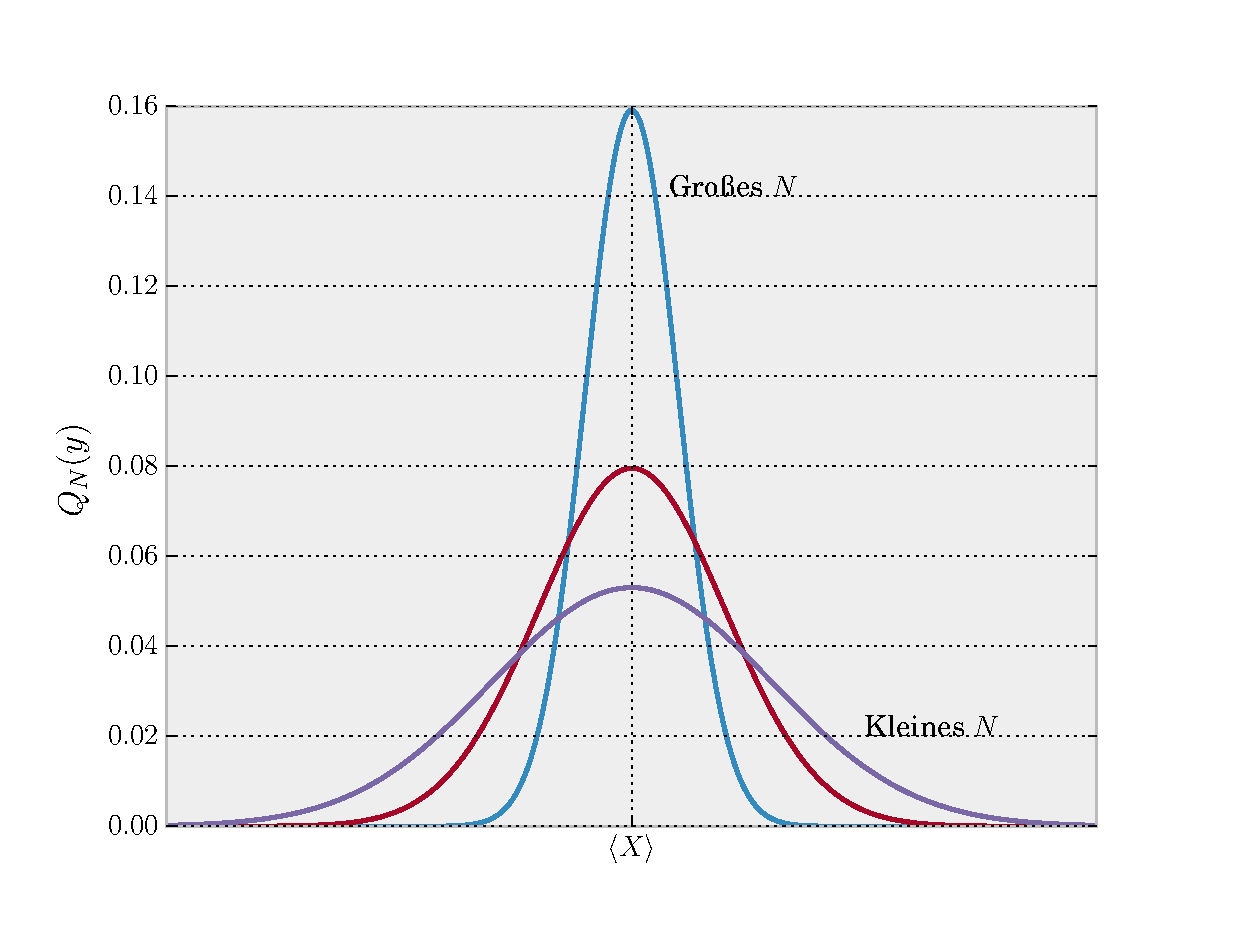
\includegraphics[width=0.8\textwidth]{./figures/first.eps}
  \caption{Normalverteilung, $Y=\Braket{X} \pm \frac{\Delta X}{\sqrt{N}} $}
  \label{fig:first}
\end{figure}
\section{Klassische Physik}
\begin{description}
  \item[N Teilchen ] Mikrozustand $(q,P) \in  \text{ Phasenraum } \simeq \R^{6n}$
  \item[Kanonische Gleichungen] \[ \dot{q}_j = \pd{H}{P_j} \quad \dot{P}_j = \pd{H}
    {\dot{q}_j}, \quad j=1,...,3N \] 
  \item[Anfangsbedingung] \[ (q_0, P_0)= (q_0(t_0), P(t_0)) \implies \text{ Bahn }
    (q(t | q_0, P_0), P(t| q_0, P_0)) \] 
  \item[Kanonische Transformation ] \[ (q(t), P(t)) \iff (q(t'), P(t')) \] 
  \item[Ziel] \[ \bar{A}= \int_{}^{} d^{3N}q\, d^{3N}p\, A(q,P) P_G(q,P) \] 
    Gleichgewichtsverteilung $P_G(q,P)= $?
  \item[Unscharfe Angangsbedingung] \[ P(q,P,t_0)= P_0 (q,P) \] 
    Scharfe Anfangsbedingung: $P_0(q,P) = \delta(q-q_0) \delta (P-P_0)$.
    Differentialgleichung f\"ur $P(q,P,t)$: Liouville-Gleichung.
    \[ P(t)= P(q,P,t)\, d^{3N}q\, d^{3N}p=P(t') = P(q,P,t')\, d^{3N}q'\, d^{3N}p' \] 
  \item[Liouville-Satz] \[ d^{3N}q\, d^{3N}p = d^{3N}q'\, d^{3N}p' \quad \left[
    \text{ Jacobi-Matrix } \frac{d^{3N}q'\, d^{3N}p'}{d^{3N}q\, d^{3N}p}= 1 \right] \] 
    \[ \implies P(q(t), P(t), t)= P(q(t'), P(t'), t'), \quad
    \text{ Erhalungsgr\"o\ss{}e } \frac{dP}{dt}=0 \] 
  \item[Kettenregel] \[ \frac{d P(q(t), P(t),t)}{dt}= \pd{P}{t} + \left\{ H,P \right\} \] 
  \item[Liouville-Gleichung] \[ \pd{P}{t}= \left\{ P,H \right\} \] 
    Bedingungen f\"ur $P_G(q,P)$ (im Gleichgewicht)
    \begin{itemize}
      \item $\left\{ P_G, H \right\}=0$
      \item $P_G \ge 0$
      \item $\int_{}^{}d^{3N}q\, d^{3N}p\, P_G (q,P)=1$.
    \end{itemize}
    Superpositionsprinzip: L\"osungen $P_1,P_2 \implies P=a_1 P_1+ a_2 P_2 $
    mit $a_1,a_2 \ge 0, \quad a_1+a_2 =1$. \\
    Makrozustand: $T,V,P,... \quad  \implies P_0 \text{ oder } P_g$?\\
\end{description}
\section{Quantenmechanik}

\emph{Schwabl Kapitel 1.4,1.5.2}\\
$N $ Teilchen, Mikrozustand $\Ket{\Psi} \in \mathcal{H} \simeq \mathcal{L}_2(\R^{3N})$
\begin{align*}
  i \hbar \frac{d}{dt} \Ket{\Psi(t)} = H \Ket{\Psi(t)} \\
  \text{Anfangsbedingung } \Ket{\Psi_0} \to \Ket{\Psi(t)} \quad \text{(eindeutig)} \\
  \text{Erwartungswert } A(t)= \Braket{\Psi(t) | \hat{A} | \Psi(t)} =\Braket{\hat{A}}\\
\end{align*}
Ziel: \[ \text{Statistische Mittelung } \quad \Braket{\hat{A}} = \trace(\hat{A}\hat{\rho}_G), \quad \hat{\rho}_G=? \] 
\subsubsection*{Definition}
Statistischer Operator, Dichteoperator, Dichtematrix, ...
\begin{align*}
  \hat{\rho} & : \mathcal{H} \to  \mathcal{H}, \text{ linear } \\
  \hat{\rho} & = \hat{\rho}^+\dagger \\
  \text{positiv-semidefinit } & \Braket{\varphi | \hat{\rho}| \varphi} \ge 0 \,\forall\,\Ket{\varphi} \in \mathcal{ H} \\
  \trace \hat{\rho } & =1  &
  \text{Spektrale Zerlegung } & \begin{split}
  \hat{\rho} &=  \sum_{n}^{} p_n \Ket{n}\Bra{n} \\ &= \int_{}^{} d \lambda \Ket{\lambda}\Bra{\lambda} w(\lambda) 
  \end{split}
   \\
  \text{Dichteoperator } & \implies \begin{matrix} p_n \ge 0 \\ \sum_{n}^{} p_n =1 \\
p_n \in \R \end{matrix} 
&
\begin{matrix} 
  w(\lambda )\ge 0 \\ \int_{}^{} d \lambda w( \lambda )=1 \\ w(\lambda) \in \R 
\end{matrix} \\
  \Braket{\hat{A}}= \sum_{n}^{}p_n \Braket{n|\hat{A}|n}.
\end{align*}
\begin{description}
  \item[Reiner Zustand]: \[ p_{n_0}=1,\, p_n =0 \,\forall\, n \neq n_0, \quad  \hat{\rho}= \Ket{n_0}\Bra{n_0} \implies \hat{\rho}^2=\hat{\rho} \]  
  \item[Gemisch]: $p_n \neq 0 $ f\"ur 2 oder mehr $n$.
    \begin{itemize}
      \item Verschr\"ankte Zust\"ande
      \item Statistisches Gemisch
    \end{itemize}
  \item[Spektrale Zerlegung] \begin{align*}
    \hat{A} &= \sum_{\alpha}^{}a_ \alpha \Ket{\alpha}\Bra{\alpha} \\
    \Braket{A}&= \sum_{n}^{}p_n \sum_{\alpha}^{}a_ \alpha \abs{\Braket{n|\alpha}}^2
    = \sum_{n}^{}\sum_{\alpha}^{} \underset{\text{Stat. Zufall}}{p_n} \underset{\text{Q.M. Zufall}}{\abs{\Braket{n|\alpha}}^2} a_ \alpha
  \end{align*}
  % TODO: Fig 4
  \[ \text{Gemisch: 2 Quellen: } I_1, \theta_1, \quad I_2, \theta_2 \implies 
  I'= I_1 ( \cos{\theta_1})^2 + I_2 (\cos{\theta_2})^2 \] 
  \[ p_1 = \frac{I_1}{I_1 + I_2}, \quad p_2 = \frac{I_2}{I_1 + I_2} \] 
\end{description}
\subsection*{Von Neumann Gleichung}
\[ i \hbar \frac{d\hat{\rho}}{dt} = \left[ H, \hat{\rho} \right] \] 
\begin{itemize}
  \item Anfangsbedingung $\hat{\rho}_0 \to  \hat{\rho}(t)$
  \item Gleichgewicht: \[ \frac{d \hat{\rho}}{dt}=0 \implies  \left[ H, \hat{\rho} \right]=0  \] 
  \item Superpositionsprinzip $\rho= a_1 \rho_1 + a_2 \rho_2 \text{ mit }
    a_1, a_2 \ge 0, \text{ und } a_1+a_2 =1 $
  \item Im Gleichgewicht: \[ \hat{\rho}_G = \sum_{n}^{} p_n \Ket{E_n}\Bra{E_n}
    = \int_{}^{} dE\, w(E)\Ket{E}\Bra{E} \quad \text{ mit }
    H \Ket{E}= E \Ket{E}\] 
  \item Isoliertes System: \[ p_n = \frac{1}{Z_n} \text{ f\"ur } E_n = E_0,
    \quad Z_n= \text{ Entartung des Niveaus } E_0 \] 
    % TODO: Fig 5
  \item Geschlossenes System: \[ p_n = \frac{1}{Z} e^{-\beta E_n} \text{ mit } 
    \beta= \frac{1}{k_B T}, \quad Z=\sum_{n}^{} e^{-\beta E_n} \] 
\end{itemize}

\subsection*{Entropie und Ensemble}
\emph{Schwabl Kapitel 2.1-2.5}\\
\begin{description}
  \item[Definition] Entropie (Quantenstatistik) \\
    \[ S =-k_B \trace(\hat{\rho} \ln{\hat{\rho}}) \quad k_B = k = 
      \text{ Boltzmann-Konstante }
    \approx \SI{1,38e-23}{\joule\per\kelvin} \] 
  \item[Eigenschaften] 
    \begin{align*}
      \hat{\rho} = \sum_{n}^{} p_n \Ket{n}\Bra{n} && p_n \ge 0 && \sum_{n}^{} p_n = 1 \\
      S(\left\{ p_n \right\}) = -k_B \sum_{n}^{} p_n \ln{p_n}
    \end{align*}
    Hinweise: \begin{align*}
      \trace \hat{A} = \sum_{n}^{} \Braket{n | \hat{A}|n} && f(\hat{\rho})= 
      \sum_{n}^{} f( p_n) \Ket{n}\Bra{n} \\
      e^{\hat{A}}= \sum_{n=0}^{ \oo } \frac{1}{n!}\hat{A}^n
    \end{align*}

    Die Entropie ist also \"uber die Diagonalemente der Dichtematrix in
    diagonalisierter Form berechenbar. Dies ist wohldefiniert, da jede
    Dichtematrix diagonalisiert werden kann.

    Extrema mit Nebenbedingung $\sum_{n}^{} p_n = 1$
    \begin{itemize}
      \item Minimum $S=0$ f\"ur einen reinen Zustand ($p_{n_0}=1, p_n =0
        \quad\forall\, n \neq n_0$)
      \item Maximum $S= k_B \ln{M}$ f\"ur $p_n = \frac{1}{M} \quad\forall\, 1,...,M$.
    \end{itemize}
    Die Entropie ist maximal f\"ur Unkenntnis \"uber den Zustand des Systems
    (Auch ma\ss{} f\"ur Unordnung).
  \item[Extensivit\"at] \[ \mathcal{H}= \mathcal{H}_A \otimes \mathcal{H}_B,
  \quad \hat{\rho} = \hat{\rho}_A \otimes  \hat{\rho}_B \] 
  \begin{align*}
    \hat{\rho}_A \to  \hat{\rho}_A \otimes  \hat{I}_B  \\
    \hat{\rho}_{\hat{B}} \to  \hat{I}_A \otimes  \hat{\rho}_B \\
    \implies \left[ \hat{\rho}_A, \hat{\rho}_B  \right]= 0
  \end{align*}
  \begin{align*}
    S & = -k_B \trace( \hat{\rho} \ln{\hat{\rho}})  \\
      & =  -k_B \trace \left[ (\hat{\rho}_A \otimes \hat{\rho_B}) 
  \ln{(\hat{\rho}_A \otimes \hat{\rho}_B)}  \right]  \\
  & = -k_B \trace (\hat{\rho}_A \ln{ \hat{\rho}_A}) - k_B \trace
    (\hat{\rho}_B \ln{ \hat{\rho}_B}) = S_A + S_B
  \end{align*}
  Nebenbedingung

  \[ S \le S_A + S_B \] (z.B. verschr\"ankte Systeme)
\item[Beispiel] System von $N$ Spins $S$ ($\vec{S}^2 =  S(S+1)$). \\
  Hilbert-Raum f\"ur einen Spin $= \mathcal{H}_1 = \C^{2S+1}$.
  Gesamter Hilbert-Raum \[ \mathcal{H} = \bigotimes_{i=1}^{N} \mathcal{H}_i \] 
  \[ \operatorname{dim} \mathcal{H} = (2S+1)^N = M \] 
  \begin{itemize}
    \item Minimum $S=0$ z.B. f\"ur $\Ket{\Psi} = \Ket{ \uparrow, \uparrow, \uparrow, \ldots, \uparrow}$.
    \item Maximum $S= k_B \ln{M}$ f\"ur $\hat{\rho}= \frac{1}{n} \hat{I}=
      k_B n \ln{(2S+1)}$
  \end{itemize}
\item[Gleichgewicht]
  \begin{align*}
    0= \frac{d \rho }{dt} \iff \left[ H, \hat{\rho} \right]=0 \implies 
    \rho = \sum_{m}^{} p_n \Ket{E_n} \Bra{E_n} \\
    \implies E = \Braket{\hat{H}} = \trace (\hat{\rho} \hat{H})
    = \sum_{n}^{} p_n E_n
  \end{align*}
  \begin{align*}
    \rho \Ket{E_n} = p_n \Ket{E_n} \\
    H \Ket{E_n} = E_n \Ket{E_n}
  \end{align*}
\end{description}
\begin{description}
  \item[Definition]  Statistisches Ensemble oder Gesamtheit \\
    Sie ist eine Gewichtete Menge der Mikrozust\"ande, die einen 
    Makrozustand entsprechen.
    \begin{align*}
      \left\{ ( \Ket{N}, p_n) \right\} \equiv \hat{\rho} = \sum_{n}^{} p_n
      \Ket{n} \Bra{n} 
    \end{align*}
\end{description}
\subsection*{Zentrales Postulat der statistischen Physik}
System mit $N\to \infty$ Freiheitsgraden im Gleichgewicht.
\begin{itemize}
  \item $S$ ist maximal f\"ur einen gegebenen Makrozustand. Das erlaubt uns
    eine eindeutige bestimmung des statistischen Operators $\hat{\rho}$.
  \item Statistische Mittelungen der Observablen erf\"ullen die Makroskopischen
    Gesetze der Thermodynamik.
    %
    \begin{align*}
      S = -k_B \trace \hat{\rho}_B = - k_B \Braket{\ln{\hat{\rho}_G}} \\
    \end{align*}
    %    
    \begin{align*}
      \Braket{\hat{\cal{O}}}= \trace (\hat{\rho}_G \mathcal{O}) &&
      U = \Braket{\hat{H}}
    \end{align*}

\end{itemize}
\begin{description}
  \item[Definition] Entropie (Thermodynamik) \\
    Wir betrachten ein System in einem Bad, mit welchem es Energie austauschen
    kann. Eine ideelle Situation, in welcher alle Prozesse die wir betrachten 
    reversibel sind. 
    \begin{align*}
      dS = \frac{\delta Q}{T}
    \end{align*}
    Zustandsfunktion oder Thermodynaische Variable.
    \begin{itemize}
      \item Extensiv
      \item monoton steigend $\pd{S}{E} > 0$
      \item $ \lim_{T \to 0} \frac{S}{N} = 0$.
    \end{itemize}
\end{description}
\begin{description}
  \item[Nebenbedingung] F\"ur bestimmte Modelle statistische Entropie nicht
    gleich der thermodynamischen Entropie, das bedeutet das Modell ist nicht
    physikalisch. Eigentlich hat man in den letzten 100 Jahren in denen man
    Forschung betreibt kein Problem gefunden, das man nicht l\"osen konnte.
    Es gibt verschiedene Situationen in derr Praxis, in denen man die Makrozust\"ande
    beschreibt. 
\end{description}
\subsection*{Mikrokanonisches Ensemble}
Es beschreibt ein isoliertes System.
\begin{description}
  \item[Freie thermodynamische Variablen] $ $ 
    \begin{itemize}
      \item Teilchenzahl $N$
      \item Volumen $V$
      \item Magnetisierung $M$
      \item Energie $E$
    \end{itemize}
  \item[Zustandsfunktion] Druck $P(N,V,E)$
  \item[Maximierung der Entropie] 
    \begin{align*}
      \hat{\rho} & = \subset P_E P_N \ldots \\
      \hat{\rho} & ~ \delta(\hat{H} - E) \delta (\hat{N} - N)
    \end{align*}
\end{description}
\subsection*{Kanonisches Ensemble}
Beschreibt ein geschlossenes System.
\begin{description}
  \item[Freie thermodynamische Variablen] $ $
    \begin{itemize}
      \item Temperatur $T$
      \item $N, V, M$
    \end{itemize}
  \item[Zustandsfunktionen] $E(T, N, V)$
  \item [Maximum der Entropie] 
    F\"ur feste $T, N, V, \ldots$
    \begin{align*}
      \hat{\rho} = \frac{1}{Z} e^{- \beta \hat{H} } \hat{P}_N \ldots && 
      \beta = \frac{1}{k_B T}
    \end{align*}
  \item[Zustandsumme]
    \begin{align*}
      Z= \trace e^{- \beta \hat{H}}
    \end{align*}
\end{description}

\subsection*{Gro\ss{}kanonisches Ensemble}
Beschreibt ein offenes System
\begin{description}
  \item[Freie Thermodynamische Variablen]  $ $
    \begin{itemize}
      \item Chemisches Potential $\mu$
      \item $T, V, \ldots$
    \end{itemize}
  \item[Zustandsfunktionen] $N(T, \mu, V)$
  \item[Maximum der Entropie] f\"ur feste $T, \mu, V$ falls
    \begin{align*}
      \hat{\rho}_G = \frac{1}{Z_{GK}} e^{-\beta(\hat{H}- \mu \hat{N})} P
    \end{align*}
  \item[Gro\ss{}kanonische Zustandssumme] $Z_{GK} 
    \trace e^{-\beta(\hat{H}- \mu \hat{N})} $
\end{description}
\subsection*{Viele weitere Ensembles}
Zu jeder intensiven Variable gibt es eine Extensive Variable(Observable).

\begin{center}
  \begin{tikzpicture}
    \matrix (m) [matrix of math nodes,column sep=6em,
      column 1/.style={anchor=base east},
      column 2/.style={anchor=base west}
    ] 
    {
      \underset{\text{Intensive Variable}}{\text{\"Au\ss{}eres Feld}} & 
      \underset{\text{Extensive Variable}}{\text{Observable}} \\
      y & x \\
      \hat{\rho}_G ~ e^{- \beta y \hat{x}} & \hat{\rho}_G ~ 
      P_x ~ \delta (\hat{x} -x ) \\
      \text{Beispiele} \\
      M & N \\
      P & V \\
      H & M \\
    \text{Magnetfeld} & \text{Magnetisierung} \\};
  \end{tikzpicture}
\end{center}


 \section*{Mikrokanonisches Ensemble}
 Wir betrachten ein isoliertes System. Zum beispiel ein Gas in einem Beh\"alter
 welcher isoliert ist. Energie und Teilchenzahl sind fest. Genauso das Volumen.
 Eine \"Ahnliche Situation w\"are auch ein magnetisches Material. Die isolation
 w\"are hier ein Material welches keine magnetischen Felder durchl\"asst.
 Typisch f\"ur das isolierte System ist, dass die Energie eine kontrollierbare
 Variable ist.

 Es gibt also eine Freie thermodynamische Variable $E$. Die erlaubten 
 Mikrozust\"ande sind die Eigenzust\"ande des Hamilton-Operators $H$ zur
 Energie $E$.
 Das Ziel ist nun die mikrozust\"ande zu beschreiben und die makroskopischen
 Variablen zu berechnen. Man braucht dazu den statistischen Operator.
 \begin{description}
   \item[Diskretes Eigenspektrum] 
     \begin{align*}
       \hat{\rho} = \sum_{n}^{} p_n \Ket{n}\Bra{n} \quad : \quad \mathcal{H} \to 
       \mathcal{H} && p_n =0 \quad\forall\, n \text{ mit } E_n \neq E \\
       \hat{\rho}= \sum_{n=1}^{w(E)} p_n \Ket{n}\Bra{n} &&
       w(E) = \text{ Entartung der Eigenergie } E
     \end{align*}
     Wir verwenden das Postulat der maximierung der Entropie:
     \begin{align*}
       S(E)= -k_B \sum_{n=1}^{w(E)} p_n \ln{p_n}, && 
       \sum_{n=1}^{w(E)} p_n = 1 
     \end{align*}
     \begin{align*}
       0  &= \pd{S}{p_n} - \lambda \pd{}{p_n} 
       \left( \sum_{n=1}^{w(E)} p_m -1 \right)  \\
       & = -k_B \left( \ln{p_n} +1 \right) - \lambda \Forall 1 ,\dotsc, w(E) \\
     \end{align*}

     \begin{align*}
       \text{ Extrema f\"ur }      
       & \implies p_n = e^{-\frac{\lambda}{k_B} - 1} \implies p_n = \frac{1}{w(E)} \\
       & \implies S(E) = k_B \ln{(w(E))} \text{ ist auch ein Maximum }
     \end{align*}

   \item[Dichteoperator im Gleichgewicht]
     \begin{align*}
       \hat{\rho}_G = \sum_{n=1}^{w(E)} \frac{1}{w(E)} \Ket{n}\Bra{n} =
       \frac{1}{w(E)} P_E = \frac{1}{w(E)} \delta(H-E) & \\
     \end{align*}
     \begin{align*}
       \trace \hat{\rho}_G = 1 && \trace P_E = w(E) \\
     \end{align*}

   \item[Kontinuierliches Spektrum]
     \begin{flalign*}
       \hat{\rho} &= \int_{}^{} d\lambda\, \Ket{\lambda}\Bra{\lambda} p(\lambda) \\
       N(E) &= \text{ Anzahl der Zust\"ande mit einer Eigenenergie } \le E
     \end{flalign*}
     Hinweis: F\"ur ein diskretes System von Eigenzust\"anden
     f\"ur ein kontinuerliches Spektrum kann man die Anzahl der Eigenzust\"ande 
     kleiner Als $w$ definieren.
     \begin{align*}
       w(E) &= \frac{dN}{dE} = \text{ Zustandsdichte } \\ & \implies w(E) \Delta E
       = \text{ Anzahl der Eigenzust\"ande in } \left[ E, E+ \Delta E \right] \\
       S(E) &= k_B \ln{(w(E) \Delta E)} \\
       \hat{\rho} &= \frac{1}{w(E)} \delta(H-E) 
     \end{align*}
 \end{description}
 \subsection*{Thermodynamische Variablen}
 Man macht eine Statistische Mittelung
 \begin{align*}
   \Braket{\hat{\cal{O}}} = \trace (\hat{\rho}_G \hat{\cal{O}})
 \end{align*}
 \begin{description}
   \item[Beispiele] 
     \begin{align*}
      \text{Innere Energie: } U= \Braket{H} = E \\
      \text{Magnetisierung: } M_z = \Braket{S_z} \\
     \end{align*}
   \item[Thermodynamischer Limes] ($N \to \infty$)
   \item[Definition] Temperatur
     \begin{align*}
       \frac{1}{T} = \left( \pd{S}{E} \right)_x
     \end{align*}
   \item[Definition] Konjugierte Variablen \\
     Beispiele: 
     \begin{align*}
       x = \begin{Bmatrix} 
         M \xleftrightarrow{\hspace{1cm}}  H \\ 
         N \xleftrightarrow{\hspace{1cm}}  M \\
         V \xleftrightarrow{\hspace{1cm}} P 
     \end{Bmatrix} y
     \end{align*}
     %
     \begin{align*}
       S(E,X) && y = \pm  T \left( \pd{S}{X} \right)_E
     \end{align*}
     %
   \item[Statistische Physik] $ $ \\
     \begin{align*}
       \text{Extensive Observable } \hat{x}, \quad && [\hat{x}, \hat{H}]
       \xrightarrow{ N \gg 1} N^0, n^{-1} \\
       \implies \Braket{\hat{x}} = x && S(E,X) = k_B \ln{ w(E,X)} \\
     \end{align*}
 \end{description}
\subsection*{Beispiel: System von nicht-wechselwirkenden Spins}
\begin{align*}
  N \text{ Spins } s=1, && H = \sum_{i=1}^{ N } H_i = J \sum_{i=1}^{N} S_{iz}^z
  \quad (J>0) \\
\end{align*}

Eigenzust\"ande: 

\begin{align*}
  \text{1 Teilchen } & \begin{cases}
    H_i \Ket{M_j} = J S_{j z}^z \Ket{m_j} = J \hbar^2 m_j^2 \\
    S_{zj} \Ket{m_j} = \hbar m_j \Ket{m_j} &  m _j = -1,0,1 \\
  \end{cases} \\
  \text{$N$ Teilchen } & \begin{cases}
    \text{Dim } \mathcal{H} = 3^N \\ %REALLY? \\
    \Ket{ \left\{ m_j \right\} }= \Ket{m_j} \otimes \Ket{m_j} \otimes  \ldots 
      \otimes  \Ket{m_N} \\
      E(\left\{ M_j \right\})= J \sum_{j=1}^{N}m_j^2 \\
      S_z \Ket{ \left\{ m_j \right\} }= {\sum_{j}^{} m_j } & M=\sum_{j}^{}
      m_j
      \Ket{ \left\{ m_j \right\} }
  \end{cases} \\
  & H\Ket{ \left\{ m_j \right\} } = E (\left\{ m_j \right\}) \Ket{ \left\{ m_j \right\} }
\end{align*}

\begin{description}
  \item[Problem]  Entartung $w(E,M)$ \\
    \begin{align*}
      N_+ & = \text{ Anzahl der Spins mit } m_j = +1 \text{ in } \left\{ m_j \right\}\\
      N_0 & = \text{ Anzahl der Spins mit } m_j = +0 \text{ in } \left\{ m_j \right\}\\
      N_- & = \text{ Anzahl der Spins mit } m_j = -1 \text{ in } \left\{ m_j \right\}\\
    \end{align*}

    \begin{align*}
      \implies \begin{cases}
        E = J (N_+ + N_-) \\
        M = N_+ - N_- \\
        N = N_+ +N_- + N_0 \\
      \end{cases}
      \implies \begin{cases}
        N_+ = \frac{R+M}{L} =  \frac{r+m}{ L}N \\
        N_- = \frac{R-M}{L} = \frac{r - m}{ L} N\\
        N_0 = N-R = (1- r ) N \\
      \end{cases}
    \end{align*}

    \begin{align*}
      \text{Energie pro Spin ist } r= \frac{R}{N}= \frac{E}{NJ} \quad \in [0, 1] \\
      \text{Magnetisierung pro Spin } m = \frac{M}{N} \quad \in [-1, 1]
    \end{align*}

    Problem: $N_+$ unterscheidbare Zust\"ande $m_j= +1$ auf $N$ Spins verteilen.

    \begin{align*}
    & \implies \begin{pmatrix} N \\ N_+ \end{pmatrix} = \frac{N!}{N_+!(N-N_+)!}
      \text{ M\"oglichkeiten }  \\
      \end{align*}

      Danach: $N_-$ unterscheidbare Zust\"ande auf $N-N_+$ Spins mit
      $m_j = -1$ verteilen.
      \begin{align*}
      \implies \begin{pmatrix} N-N_+ \\ N_- \end{pmatrix} \text{ Moeglichkeiten} 
      \end{align*}

      Also insgesamt:
      \begin{align*}
       w(E,M) & = w(N_+, N_-) \\
      & = 
      \begin{pmatrix} N \\ N_+ 
      \end{pmatrix}  
      \begin{pmatrix} N-N_+ \\ N_- 
      \end{pmatrix} \\ & = \frac{N!}{N_+! N_-! N_0!} 
      \end{align*}

      Damit folgt die Entropie:
      \begin{align*}
        \begin{split}
         S(E,M) & = S(N_+, N_-) \\ &= k_B \ln{}\left( 
        \frac{N!}{N_+! N_-! N_0! }\right) 
      \end{split}
    \end{align*}
  Annahme: $N, N_+, N_0, N_- \gg 1$ aber
    
    \begin{align*}
      & \frac{N_+}{N}, \frac{N_-}{N}, \frac{N_0}{N} \text{ fest und endlich } \\
      \iff & m,n \text{ fest und endlich} \\
      \iff & M,E \text{ sind extensiv } (M,E \propto N)
    \end{align*}
    Stirling Formel \begin{align*}
      & \ln{N!} \approx N \ln{N} - N \\
      \implies & S(E, M) = k_B N f(r, m) \\
      f(r, m ) & = - \left[ \frac{r+m}{2} \ln{(r+m)} + \frac{r - m}{2}
    \ln{\frac{(r - m)}{2}} + (1-r) \ln{(1 - r)} \right]
    \end{align*}
  \item[Temperatur]
    \begin{align*}
      \frac{1}{T} = \left( \pd{S}{E}  \right)_M = \frac{k_B}{J} 
      \ln{\left( \frac{2 (1-r)}{ \sqrt{r^2 - m^2}} \right)}
    \end{align*}
  \item[Ohne Magnetisierung] $M=0$ genau dann, wenn $m=0$.
    \begin{align*}
      S(E) = - k N [ r \ln{\frac{r}{2}} + (1-r) \ln{(1-r)}] \\
    \end{align*}
    %
    \begin{align*}
      \frac{1}{T} = \frac{k_B}{ J } \ln{\left( \frac{2 ( 1-r)}{r} \right) }
       \begin{cases}
         > 0 & \text{ falls } 0 < r < \frac{2}{3} \\
         < 0 & \text{ falls }\frac{2}{3} < r < 1 \\
      \end{cases}
    \end{align*}
    \begin{align*}
      \implies  r (T) &= \frac{2}{e^{\beta J }+2 }, \quad  \beta= \frac{1}{k_B T} \\
                E(T)  &= NJ \frac{2}{e^{\beta J}} \frac{2}{e^{\beta J} + 2} \\
                S(T)  &= k N \left[ \frac{2}{e^{\beta J} + 2} \ln{(e^{\beta J} + 2)}
    - \frac{1}{e^{-\beta J} + 2} \ln{ \left( 1+ 2 e^{-\beta J} \right) }\right]
    \end{align*}
  \item[Diskussion] $ $  \\
    Tiefe Temperaturen \begin{align*}
      k_B T \ll J \iff \beta J \longrightarrow \infty \quad \implies \begin{cases}
        E \longrightarrow 0 \\ S \longrightarrow 0
      \end{cases}
    \end{align*}
    Nebenbedingung f\"ur $J < 0$: 
    \begin{align*}
      \implies  \begin{cases}
        E = N J \\
        S = k_B N \ln{(z)}
      \end{cases}
    \end{align*}

    Hohe Temperatur $k_B T \gg J$

    \begin{align*}
      \iff \beta J \longrightarrow  0 \implies 
      \begin{cases}
        E = \frac{2}{3} N J \\
        S = \frac{1}{3} k_B N \ln{(3)}
      \end{cases}
    \end{align*}
\end{description}
\subsection*{Kanonisches Ensemble}
\emph{Schwabl Kapitel 2.6} \\
Schwabl nimmt an, dass man das gesamte System mikrokanonisch behandeln kann.
$\hat{\rho} \propto \delta (\hat{H} -E)$. Das innere Teilsystem 2 ist
viel kleiner als das \"au\ss{}ere Teilsystem 1. Also ist auch die \"anderung
der Energie des Systems 1 $\Delta E_1 \gg \Delta E_2$. Man benutzt dann
das Prinzip der maximierung der Entropie $S$ woraus folgt, dass
%
\begin{align*}
  \hat{\rho}_2 = e^{- \hat{H}_2 / (k_B T_2) }
\end{align*}
%
Quantenmechanik Anmerkung:
%
\begin{align*}
  \mathcal{H} = \mathcal{H}_1 \otimes \mathcal{ H}_2 && \text{ Basis } 
  \left\{ \Ket{n_1} \otimes \Ket{n_2} \right\} \text{ von } H
\end{align*}
%
\begin{align*}
  \trace \hat{A} = \sum_{n}^{} \Braket{n | \hat{ A} | n} = 
  \sum_{n_1}^{} \sum_{n_2}^{} \Braket{n_1 n_2 | \hat{A} | n_1 n_2} 
\end{align*}
%
%
\begin{align*}
  \hat{A}_1 & = \trace_{\mathcal{H}_1} \hat{A} = \sum_{n_2}^{} \Braket{n_2 | \hat{A} | n_2} \\
            & = \sum_{n_2}^{} \sum_{n_1}^{} \sum_{n_1'}^{} 
  \Braket{ n_1 n_2 | \hat{A} | n_1' n_2} \Ket{n_1} \Bra{n_1'}
\end{align*}
%

%

%
\begin{align*}
  \hat{\rho}_1 = \trace_{\mathcal{H}_1} \hat{\rho} \implies S_1 (E_1) = 
  \frac{1}{T_1} = \left( \pd{S_1}{E_1} \right) = \frac{1}{T} .
\end{align*}
%

Wir betrachten ein geschlossenes System im Gleichgewicht mit W\"armebad der 
Temperatur $T$. Was ist der statistische Operator $\hat{\rho}$ ?

\begin{description}
  \item[Definition]  Freie Energie (Thermodynamik, makroskopisch)
    %
    \begin{align*}
      F(T) = U(S(T)) - T S(T)
    \end{align*}
    Legendre-Transformation
    %
    \begin{align*}
      \frac{1}{T} = \left( \pd{S}{E} \right)_X \iff T_X =
      \left( \pd{E}{S} \right)_X \\
      \implies S = - \left( \pd{F}{T} \right)_X
    \end{align*}
    %
  \item[Postulat] Im thermischen Gleichgewicht ist die Entropie maximal. 
    Dies gilt genau dann wenn die freie Energie minimal ist.
    %
  \item[Definition] Funktional der freien Energie In der 
    mikroskopischen statistischen Physik.
    % 0
    \begin{align*}
      F[\hat{\rho}] & = E[\hat{\rho}] - T S [\hat{\rho}] \\
                    & \text{mit } E [\hat{\rho}] = \Braket{\hat{ \mathcal{H}}}
      = \trace (\hat{\rho} \hat{ \mathcal{H}})
    \end{align*}
    %
  \item[Minimierung von ] $F[\hat{\rho}]$ \\
    Variationsrechnung $\delta F= 0 \quad\forall\, \delta \hat{\rho}$
    \begin{enumerate}
      \item %
      \begin{align*}
          \delta F & = F \left( \hat{\rho} + \delta \hat{ \rho} \right) -
          F \left( \hat{\rho} \right) \\ & = \trace (H \delta \hat{\rho}) 
        + k_B T \trace (\delta \hat{\rho} \ln{\hat{\rho}}) + k_B T \trace
        \delta \hat{\rho} \\ & = \trace ( ( H+ k_B T \ln{ \hat{\rho}}) \delta \hat{\rho}) \\
      \end{align*}
      Wir verwenden, dass man kompakte operatoren in der Spur vertauschen kann.
      %
      \begin{align*}
        \trace (\hat{A} \hat{B}) = \trace (\hat{B} \hat{A})  \\
        \trace \hat{\rho} = 1 \implies \trace \delta \hat{\rho} = 0
      \end{align*}
      %
    \item
      %
      \begin{align*}
        \delta F = 0 \quad\forall\, \delta \hat{\rho} \implies 
        H + k_B \ln{\hat{\rho}} = c \iff
        \hat{\rho} = e^{ \frac{\hat{H}}{k_B T} } e^{ \frac{c}{ k_B T}} \\
      \end{align*}
      %
      Die folgenden drei Formeln sollte man sich merken:
      \begin{align*}
        \implies \hat{\rho} = \frac{1}{Z} e^{-\beta \hat{H}} && \beta = \frac{1}{k_B T} \\
      \end{align*}
      %
      \emph{Kanonische Zustandsumme}
      \begin{align*}
         Z = \trace e^{-\beta \hat{H}} 
      \end{align*}
      %
      Minimum von $F[\hat{\rho}] \equiv $ Freie Energie.
      %
      \begin{align*}
        F = -k_B T \ln{Z} 
      \end{align*}
      %
      Bemerkung: $\hat{\rho} = e^{-\beta \hat{H}} P_N$ %TODO
    \end{enumerate}
    Weitere thermodynamische Variablen %
    \begin{align*}
      x = \trace (\hat{\rho} \hat{x}) \text{ z.B. } M,N
    \end{align*}
    %
    %
    \begin{align*}
      \text{Thermodynamik } y = \pm \left( \pd{F}{X}  \right)_T, 
      \text{ z.B } P = - \left( \pd{F}{V} \right)_T, B = 
      \left( \pd{F}{M} \right)_T
    \end{align*}
    %
\end{description}
\subsection*{Statistische Bedeutung der W\"arme}
%
\begin{align*}
  dE & = d \trace \left( \hat{\rho} \hat{H} \right) = 
  \trace\left( d \hat{\rho} \hat{H} \right) + 
  \trace \left( \hat{\rho} d \hat{H} \right)  \\
  dS & = -k_B d \trace \left( \hat{\rho} \ln{ \hat{\rho}} \right) = 
  - k_B \trace \left( d \hat{\rho} \ln{ \hat{\rho}} \right) - k_B \trace d \hat{\rho} \\
   & \underset{\hat{\rho} = \frac{1}{z } e^{- \beta \hat{ H}}}{=} 
  \frac{1}{T} \trace (d\rho \hat{H}) \\
\implies & dE = T dS + \trace \left( \hat{\rho} d \hat{H} \right).
\end{align*}
\emph{1. Hauptsatz der Thermodynamik} 
%
\begin{align*}
  dV = \delta Q + \delta A
\end{align*}
%
\begin{itemize}
  \item Reversibler Prozess
    %
    \begin{align*}
      \delta Q & = T dS = \trace \left( d \hat{\rho} \hat{H} \right) \\
      \delta A & = \trace \left( \hat{\rho} d \hat{H} \right)
      \implies & \text{ \"Anderung der W\"arme $\equiv$ 
    \"Anderung der Wahrscheinlichkeit der Mikrozust\"ande}
    \end{align*}
    %
\end{itemize}
\subsection*{Energiefluktuationen}
Wahrscheinlichkeit f\"ur Mikrozustand mit Energie $E$.
Diskretes Spektrum 
%
\begin{align*}
  P(E) = 
  \begin{cases}
    \frac{1}{Z} e ^{-\beta E} & \text{ Falls Eigenenergie $E$ existiert} \\
    0                         & \text{ Falls Eigenenergie $E$ nicht existiert} \\
  \end{cases}
  \end{align*}
%
Kontinuerliches Spektrum 
%
\begin{align*}
  P(E) & = W(E) \Delta E \\
  W(E) & = w(E) \frac{1}{Z} e^{-\beta E} \\
\end{align*}
%
Definition einiger Gr\"o\ss{}en
\begin{itemize}
  \item Mittelwert 
    %
    \begin{align*}
      \bar{E} = \int_{}^{} \d{E} w(E) E = \Braket{\hat{H}} = U
    \end{align*}
    Nebenbedingung
    %
    \begin{align*}
      \Braket{H} = -\pd{}{\beta} \ln{Z} 
    \end{align*}
  \item Schwankungsquadrat 
    %
    \begin{align*}
      \Delta E ^2 = \int_{}^{} \d{E} W(E) \left( E- \bar{E} \right) ^2 
      = \Braket{\hat{H}^2} - \Braket{\hat{H}} ^2
    \end{align*}
    %
    Nebenbedingung
    %
    \begin{align*}
      \Delta E^2 = - \pd{\bar{E}}{\beta} = - \pd{\Braket{\hat{H}}}{\beta}
    \end{align*}
    %
  \item W\"armekapazit\"at 
    %
    \begin{align*}
      C_x = \left( \frac{dU}{dT} \right)_x = \frac{1}{k_B T^2} \Delta E^2 &&
      \beta = \frac{1}{k_B T}
    \end{align*}
    %
    3. Hauptsatz
    %
    \begin{align*}
      \lim_{T \to  0} C_x = 0 \implies \lim_{T\to  0 } \Delta E^2 = 0 
    \end{align*}
    %
\end{itemize}
\subsection*{Relation mit dem mikrokanonischen Ensemble}
Experiment: $U$ und $C_x$ sind extensiv. Das bedeutete mathematisch, dass
$U$ und $C_x$ proportional zur Teilchenzahl $N$ sind. Das bedeutet auch, dass
der Mittelwert $\bar{E}$ und das Schwankungsquadrat $\Delta E$ proportional 
zur Teilchenzahl sind. Das bedeutet f\"ur die relative Breite:
%
\begin{align*}
  \frac{\Delta E}{\bar{E}} \propto \frac{1}{\sqrt{N}} 
  \xrightarrow{\text{Thermodynamischer Limes}} 0
\end{align*}
%
% zeichnung
%
%
\begin{align*}
  P(\bar{E}) & = W(\bar{E}) \Delta E \xrightarrow{n\to\infty} 1 \\
  \text{ oder } & W(E) \to \delta(E - \bar{E})
\end{align*}
%
\"Aquivalenz der mikrokanonischen und kanonischen Ensembles im
thrmodynamischen Limes $( \frac{\Delta E}{N} \to 0)$.

\subsection*{Beispiel: Spin System}
%
\begin{align*}
  \hat{H} = J \sum_{i=1}^{N} S_{iz}^z - B \sum_{i=1}^{N} S_{iz} 
  = \sum_{i=1}^{N} H_i
\end{align*}
%
%
\begin{align*}
  \hat{\rho} = \frac{1}{z} e^{-\beta \hat{H}}  &&
  \left[ H_j, H_l \right] = 0 \quad\forall\, j,l = 1,\dotsc,N
\end{align*}
%
%
\begin{align*}
  Z = \trace_\mathcal{H} e^{-\beta \hat{H}} = \trace_{\mathcal{H}_1} e ^{-\beta \hat{H}_1} \trace
  e^{-\beta \hat{H}_2} \ldots \trace_{\mathcal{H}_N} e^{-\beta \hat{H}_N}
\end{align*}
%
%
\begin{align*}
  Z_1 = \trace_{\mathcal{H}_1} e^{-\beta \hat{H}_1} = \sum_{m_1=1,0,1}^{}
  \Braket{m_1 | e^{-\beta \hat{H}_1} | m_1} \\ \hat{H}_1 \Ket{m_1} = 
  \left( J m_1^2 - \beta m_1 \right) \Ket{m_1}
\end{align*}
%
%
\begin{align*}
  \implies & Z_1 = 1 + e^{-\beta (J+B)} + e^{-\beta (J-B)} \\
  \implies & Z = \left( 1 + e^{-\beta (J+B)} + e^{-\beta(J-B)} \right)^N
  & = \left( 1+2 e^{-\beta J} \cosh(\beta B) \right)^N
\end{align*}
%
%
\begin{align*}
  Z = \left( 1 + Z e ^{-\beta J} \cosh(\beta B) \right)^N 
\end{align*}
\emph{Freie Energie}
%
\begin{align*}
  F(T, X) = - k_B T \ln{Z (T, X)} && X = V, M \\
\end{align*}
\emph{Freie Enthalpie} 
%
\begin{align*}
  G (T, Y) = -k_B T \ln{Z(T, X)} && y = P, B
\end{align*}
\emph{Legendre Transformation}
%
\begin{align*}
  G(T, B) = F (T, M(T, B)) - M(T,B) B
\end{align*}
%
\begin{align*}
  B = \left( \pd{F}{M} \right)_T && M = - \left( \pd{G}{B} \right)_T
\end{align*}
%
%
\begin{align*}
  \implies G(T,B) = -k_B T N \ln{\left( 1+ 2 e^{- \beta J} \cosh{\beta B} \right)}
\end{align*}
%

\begin{description}
  \item[Magnetisierung] 
    %
    \begin{align*}
      M & = \Braket{S_z} = \frac{1}{Z} \trace (e^{-\beta \hat{H}} \hat{S}_z) \\
        & = \frac{1}{\beta} \pd{\ln{ Z}}{\beta} \\
        & = N \frac{2 e^{-\beta J} \sinh(\beta B)}{1 + 2 e^{-\beta J} \cosh
    (\beta B)}
    \end{align*}
    anmerkung:
    %
    \begin{align*}
      Z = \trace e^{-\beta H} && H = J \sum_{i}^{} \hat{S}_{iz}^z - B \sum_{i}^{}
      S_{iz}
    \end{align*}
    %
    \begin{itemize}
      \item Tiefe Temperatur $k T \ll J, \abs{B}$
        \begin{itemize}
          \item Falls $\abs{B} < J$ so geht $M \to 0$ \\
          \item Falls $\abs{B} < J$ so geht $M \to \tanh(\beta B) \to N \sign(B)$
            Im Grundzustand $ \Ket{m_1 = \sign B}$.
        \end{itemize}
    \item Hohe Temperatur $k T \gg J, \abs{B}$ \\
        %
        \begin{theorem*}[ Curie-Gesetz ]
            \begin{align*}
                M = N \frac{2}{3} \frac{B}{k_B T}
            \end{align*}
        \end{theorem*}

        %
        
    \end{itemize}
\end{description}
\subsection*{Gro\ss{}kanonisches Ensemble}
\emph{Schwabl Kapitel 2.7} \\
Wir haben einen offenen Beh\"alter, in dem sich ein Untersystem befindet.
Man kontrolliert nicht die Teilchenzahl und die Energie, sondern nur die TEmperatur
und das chemische Potential.
Es handelt sich also um ein offenses System im Gleichgewicht mit
\begin{itemize}
  \item Einem W\"armebad bei Temperatur $T$.
  \item Einem Teilchenreservoir mit chemischem Potential $\mu$.
\end{itemize}
\begin{beispiel} Wasserspiegel
    
\end{beispiel}

% insert graphics here
\begin{definition} Gro\ss{}kanonisches Potential der Thermodynamik
    %
    \begin{align*}
      \Phi(T, \mu) = U\left( S (T, \mu), N(T, \mu) \right) - 
      T S(T, \mu)  - \mu N(T, \mu) 
    \end{align*}
    %
    %
    \begin{align*}
      T = \left( \pd{U}{S} \right)_{X, N} && \mu = \left( \pd{ U}{N} \right)_{X, T} \\
      S = - \left( \pd{F}{T} \right)_{X, \mu} && N = -\left( \pd{\Phi}{\mu} \right)_{X, T} \\
    \end{align*}
\end{definition}

%
\begin{postulat}
    Thermodynamisches Gleichgewicht besteht genau dann, wenn
    die Entropie $S$ maximal ist. Oder \"Aquivalent, das gro\ss{}kanonische
    Potential $\Phi$ minimal ist.
\end{postulat}

\begin{definition}
    Funktional des gro\ss{}kanonischen Potentials
    (Statistische Physik)
    %
    \begin{align*}
        \Phi[\hat{\rho}] = E \left[ \hat{\rho} \right] - T S [\hat{\rho}]
        - \mu N[ \hat{\rho}]
    \end{align*}
    %
    wobei %
    \begin{align*}
        N [\hat{\rho}] = \trace (\hat{\rho} \hat{N})
    \end{align*}
    %
\end{definition}
        
Wir minimieren nun $\Phi[\hat{\rho}]$ unter $\hat{\rho}$ mit
$ \trace \hat{\rho} = 1$. Daraus folgt der statistische Operator.
%
\begin{align*}
    \text{Statistischer Operator} && & \hat{\rho} = \frac{1}{Z} 
    e^{- \beta (\hat{H} - \mu \hat{N})} \\
    \text{Zustandsumme } && & Z = \trace e^{-\beta (\hat{H} - \mu \hat{N})}  \\
    \text{Gro\ss{}kanonisches Potential}  && &
    \Phi (T, \mu) = -k_B T \ln{Z} 
\end{align*}
    %
\subsection*{Kanonisch und Gro\ss{}kanonisch}

\begin{itemize}
  \item Kanonisch 
    \begin{align*}
        & \text{Hilbert-Raum f\"ur N-Teilchen} && \mathcal{H}_N. \\
        & \text{Hamilton-Operator } && H_N:\mathcal{H}_N \to \mathcal{H}_N. \\
        & \text{Statistischer Operator} && \hat{\rho}_{K, N} = \frac{1}{Z_K(N)}  
        e^{-\beta \hat{H}_N} : \mathcal{H}_N \to \mathcal{H}_N \\
               & \text{Zustandsumme } && Z_K(N)= \trace_{\mathcal{H}_N} e ^{-\beta \hat{H}_N} \\
    \end{align*}

  \item Gro\ss{}kanonisch
      \begin{align*}
          & \text{Hilbert-Raum f\"ur beliebige Teilchenzahl}  &&
          \mathcal{H} = \bigoplus_{N=0}^{\infty} \mathcal{H}_N \\
          & \text{Projektor } &&  \hat{P}_N : \mathcal{H} \to \mathcal{H}_N \\
          %
          & \text{Hamilton-Operator } &&  \hat{H}: \mathcal{H} \to \mathcal{H}, \quad
          \hat{H}_N = \hat{P}_N \hat{H} \hat{P}_N \\
          %
          & \text{Statistischer-Operator } &&
          \hat{\rho}_{GK} = \frac{1}{Z_{\text{GK}}} e^{-\beta (\hat{H} - 
          \mu \hat{N})}: \mathcal{H}\to \mathcal{H} \\
          %
          & \text{Teilchenzahl-Operator } &&  \hat{N} = \sum_{N=0}^{\infty} N
          \hat{P}_N \text{ oder } \hat{N} \Ket{\Psi} = N \Ket{\Psi}
          \quad\forall\, \Ket{\Psi} \in \mathcal{H}_N \\
          %
          & \text{Zustandsumme } &&  Z_{\text{GK}} = \trace_{\mathcal{H}} 
          e^{- \beta (\hat{H} - \mu \hat{N})}
      \end{align*}
      %
      %
      \begin{align*}
          \hat{\rho}_{N, K}& = \hat{P}_N \hat{\rho}_{\text{GK}} \hat{P}_N
          e^{- \beta \mu N} \frac{Z_{\text{GK}}}{Z_{K,N}} \\
          %
          \hat{\rho}_{\text{GK}} & = \frac{1}{Z_{\text{GK}}} \sum_{N=0}^{\infty}
          Z_K (N) \hat{\rho}_{K, N} e^{\beta \mu N} \\
          Z_{\text{GK}} (\mu)  & = \sum_{N = 0}^{ \infty} e^{\beta \mu N} Z_k(N) 
          = \trace_{\mathcal{H}} \left( e^{-\beta(\hat{H} - \mu \hat{N})}  \right) \\
          & = \sum_{N=0}^{ \infty} \trace_{\mathcal{H}_N} 
          \left( e^{-\beta(\hat{H} - \mu \hat{N})} \right)  \\
          & = \sum_{N=0}^{\infty} 
          \underbrace{\trace_{\mathcal{H}} \left( e^{-\beta \hat{H}_N} \right) e^{\beta \mu N}}_{Z_K(N)}
      \end{align*}
      %
\end{itemize}
\subsection*{Fluktuation der Teilchenzahl}
%
 Wahrscheinlichkeit daf\"ur, dass das System sich in einem Mikrozustand mit 
 $N$ Teilchen befindet.
\begin{align*}
    P(N)  & = 
     \Braket{\hat{P}_N} = \Braket{\delta (\hat{N} - N)} 
  = \frac{1}{Z_{\text{GK}}} \trace_{\mathcal{H}} = \hat{P}_N
  e ^{-\beta (\hat{H} - \mu \hat{N})} \\ & = 
  \frac{Z_K(N)}{Z_{\text{GK}}} e^{\beta M N}
\end{align*}
%
\begin{description}
  \item [Mittlere Teilchenzahl]
  %
  \begin{align*}
    \bar{N} = \Braket{\hat{N}} = \sum_{N=0}^{\infty} N P(N)
  \end{align*}
\item[Nebenbedingung]
  %
  \begin{align*}
    \Braket{\hat{N}} = \frac{1}{\beta} \pd{\ln{\hat{P}}}{\mu}
  \end{align*}
  %
\item[Fluktuationen] 

  \begin{align*}
    \Delta N^2 & = \Braket{\left( \hat{N} - \Braket{\hat{N}} \right)^2} \\ 
               & = \sum_{N = 0 }^{\infty} P(N) (N - \bar{N})^2 \propto \bar{N}
  \end{align*}
  %
  %
  \begin{align*}
    P(N) \xrightarrow{N \gg 1} \delta (N - \bar{N})
  \end{align*}
  %
  Das bedeutet die \"Aquivalenz zwischen kanonischem und gro\ss{}kanonischem
  Ensemble.
\end{description}

\begin{table}[htpb]
  \centering
  \begin{tabular}{p{4.5cm}|p{3cm}|p{3cm}|p{3cm}}
    Ensemble & mikrokanonisch & kanonisch & gro\ss{}kanonisch \\
    \hline 
    Physikalisches System & isoliert & geschlossen & offen \\
    \hline 
    Thermodynamische Variablen & $N, E$ & $T,N$ & $T, \mu$ \\
    \hline 
    Thermodynamische Funktionnen & $T, \mu$ & $E, \mu$ & $E, N$ \\ 
    \hline 
    Zustandsumme & $w(E, N) = \trace_{\mathcal{H}_{E,N}} \hat{I} = 
    \trace_{\mathcal{H}} \hat{P}_E \hat{P}_N$ & $Z_K (T, N) = 
    \trace_{\mathcal{H}_N} e ^{-\beta \hat{H}} = 
    \trace_{\mathcal{H}} e^{-\beta \hat{H}} \hat{P}_N$ & 
    $Z_{\text{GK}}(T, \mu) = \trace_{\mathcal{H}} e^{-\beta(\hat{H} -\mu \hat{N})}$ \\
    \hline 
    Statistischer Operator & 
    $ \hat{\rho} = \frac{1}{w} \hat{\rho}_E \hat{\rho}_N$ & 
    $\hat{\rho}_K = \frac{1}{Z_K} e^{-\beta \hat{H}_N}
    = \frac{1}{Z_K} \hat{\rho}_N e ^{-\beta H} \hat{\rho}_N$ & 
    $\hat{\rho}_{\text{GK}} = \frac{1}{Z_{\text{GK}}} e^{-\beta (\hat{H} - \mu \hat{N})}$ \\
    \hline 
    Thermodynamische Potentiale & $S(E, N) = k_B \ln{ w (E, N)}$ & 
    $F(T, N) = -k_B T \ln{Z_K}$ & $\Phi = -k_B T \ln{Z_{\text{GK}}}$ \\
    \hline 
  \end{tabular}
  \caption{\"Ubersicht der Ensembles der statistischen Physik}
\end{table}
%

\section*{Klassische Statistische Physik}
\emph{Schwabl Kapitel 2, Nolting Band 6 Kapitel 1}
Das Problem besteht aus Mikrozust\"anden eines Systems von $N$-Teilchen.
%

\begin{description}
  \item[Problem]
    \begin{align*}
      \text{Mikrozust\"ande } && (q,p) \in \R^{6\N} \\
      \text{Zeitmittelung} && A_z = \frac{1}{T_z} \int_{0}^{T_z} \d{t} A(q(t),p(t)) \\
      \text{Ensemblemittelung} && A_E = \int_{}^{} \d{q}\d{p} A(q,p) \rho(q,p) \\
    \end{align*}
  \item[Ergodenhypothese] %
    \begin{align*}
      A_E = \lim_{T_z\to  \infty} \lim_{N\to  \infty} A_Z
    \end{align*}
    %
\end{description}
Klassische Physik und das Postulat der statistischen Physik bestimmen 
$\rho(q,p)$ nicht. Deshalb benutzt man die Quantentheorie und das Postulat
der klassichen statistischen Physik. Auf diese Art und Weise erh\"alt man
die Quantenstatistik. Diese ergibt im klassischen Grenzfall wieder die
klassische Statistische Physik. 
\begin{description}
  \item[Klassischer Grenzfall] 
    Beispiel: Fermi-Gas mit Fermi-Temperatur $T_F$ \\
      %
      \begin{align*}
        T < T_F:& \quad \text{ Fermi-Dirac-Verteilung } f(\varepsilon)
        = \frac{1}{1 + e^{\beta(\varepsilon - \mu)}} \\
        T \gg T_F: & \quad \text{ Maxwell-Boltzmann-Verteilung} f(\varepsilon)
        = c e^{-\beta \varepsilon}
      \end{align*}
      %
      Elektronen im Metall: $T_F \approx \SI{10e3 }{\kelvin} \text{ bis } \SI{10e4}{\kelvin}$
      %
      \begin{align*}
        H_e^3 \quad: \quad T_F \approx \SI{3}{\kelvin}
      \end{align*}
      % 
      % TODO: Picture of quantum oscillators
\end{description}

\begin{description}
  \item[Mikrokanonisches Ensemble]  $(q, p ) \in \R^{6 N}$
    %
    \begin{align*}
      \rho(q, p) = \frac{1}{w(E)} \delta\left( H(q,p) - E \right)
      \frac{1}{N!} \frac{1}{h^{3N}} \\
      w(E, N) = \frac{1}{N!} \frac{1}{h^{3 N}} \int_{}^{} \d{q}\d{p}
      \delta(H(q,p)-E) \\
      \text{Entropie } S(E, N) = k_B \ln{w(E,N)} \\
    \end{align*}
    $w(t) \Delta E$ entspricht dem Phasenraumvolumen der Mikrozust\"ande mit
    Energie $m[E, E + \Delta E]$.
    % TODO: Picture of phase space
  \item[Kanonisches Ensemble] 
    %
    \begin{align*}
      \rho(q,p) = \frac{1}{Z_K} e^{-\beta H(q,p)} \frac{1}{N!} \frac{1}{h^{3N}} \\
      Z_K = \frac{1}{N!} \frac{1}{h^{3N}} \int_{}^{} \d{q} \d{p} e^{-\beta H(q,p)}
    \end{align*}
    Die freie Energie Schreibt sich als
    %
    \begin{align*}
      F(T, N) = -k_B T \ln{Z_K(T,N)}
    \end{align*}
    %
  \item[Gro\ss{}kanonisches Ensemble] 
    %
    %
    \begin{align*}
      Z_{\text{GK}} (T, \mu) & = \sum_{N=0}^{\infty} e^{\beta \mu} Z_K (T, N) \\
      & \implies \Phi(T, \mu) = -k_B T \ln{Z_{\text{GK}}(T,\mu)} \\
      \\
      \rho(q,p) & = \frac{1}{Z_{\text{GK}}} \sum_{N=0}^{\infty} e^{-\beta\left( 
      H_N(q_N,p_N) - \mu N\right)} \frac{1}{N h^{3N}} \delta(q-q_N) \delta(p-p_N)
    \end{align*}
    %
\end{description}
\begin{itemize}
  \item %
    \begin{align*}
      0 = \left\{ H,P \right\} = \left\{ H, H \right\} \dd{p}{H}
    \end{align*}
    %
  \item Entropie 
    %
    \begin{align*}
      S & \neq - k_B \int_{}^{} \d{q} \d{p} \rho(q,p) \ln{\rho(q,p)} \\
        & = -k_B \int_{}^{} \d{q} \d{p} \rho(q,p) \ln{\left( 
  \rho(q,p) N! h^{3N}\right)}
    \end{align*}
    %
  \item Mit $Z$ Zwangsbedingungen wird $6N$ zu $6N - 2Z$ und $3N$ zu $3N - Z$.
  \item Vorfaktor $h^{-3N}$
  \item Erwartungswert 
    %
    \begin{align*}
      \Braket{A} \propto \frac{h^{3N}}{h^{3N}} = 1
    \end{align*}
    %
  \item Die Entropie $S$ und die Freie Energie $F$ sind von der Form
    %
    \begin{align*}
      S(h) = S + c N \ln{h} \\
      F(h) = F + c' N \ln{h}
    \end{align*}
    Als Schlussfolgerung sind diese Werte nicht experimentell messbar.
    %
    Bemerkung: die Konstante $c'$ wiederspricht dem 3. Hauptsatz der
    Thermodynamik, aber das ist wegen des klassischen Limits kein Problem.
\end{itemize}

\begin{description}
  \item[Vorfakor $N!$] 
    In der Quantentheorie gibt es austauschsymmetrie zwischen identischen
    Teilchen.
    \begin{itemize}
      \item Erwartungswert
        %
        \begin{align*}
          \Braket{A} \propto \frac{N!}{N!} = 1
        \end{align*}
        %
      \item $S, F, \Phi \propto N$, also sind sie extensive Gr\"o\ss{}en.
    \end{itemize}
  \item[Gibbs-Paradoxon]
    Wir haben zwei urspr\"unglich getrennte Systeme die addiert werden.
    % TODO: Picture of system
    Es gibt ein Gleichgewicht, also 
    %
    \begin{align*}
      T_1 = T_2 && P_1 = P_2
    \end{align*}
    %
    F\"ur eine Mischung von 2 Gasen 
    %
    \begin{align*}
      N! \to N_1! N_2!
    \end{align*}
    %
    Mit $N$ unterscheidbare Teilchen.
  \item [Beispiel] Klassisches ideales Gas. \\
    $N$ Teilchen im Potential $V$.
    \begin{align*}
      H(\vec{r}, \vec{p}) = \sum_{i=1}^{ N} \frac{\vec{P}_i ^2}{ 2m}
      + \sum_{j = 1}^{ N} V(\vec{r}_j) \\
      V(\vec{r}) = 
      \begin{cases}
        0 & \text{f\"ur } \vec{r} \in V \\
        \infty & \text{f\"ur } \vec{r} \not\in V \\
      \end{cases}
    \end{align*}
%
    \item[Mikrokanonisches Ensemble]
      %
      \begin{align*}
        \Omega(E) = \frac{1}{N!} \frac{1}{h^{3N}} \int_{}^{} \d{^{3N} r}
        \int_{}^{} \d{^{3N} p} \quad \Theta(E - H(\vec{r}, \vec{p}))
      \end{align*}
      Wobei
      %
      \begin{align*}
        \Theta(x) = \begin{cases}
          1 & x>1 \\
          0 & x <0 \\
        \end{cases}
      \end{align*}
      Die Heaviside Theta Funktion ist.
      %
      Die Integrale stellen ein Phasenraumvolumen der Energie $< E $ dar.
      Wir werden nun diese Gr\"o\ss{}e berechnen. In diesem Integral k\"onnen
      wir anstatt \"uber $R^{3N}$ nur \"uber das Volumen integrieren.
      %
      \begin{align*}
        \Omega(E) & = \frac{1}{N!} \frac{1}{h^{3N}} \underbrace{\int_{V^N}^{} \d{^{3N} r}}_{V^N}
        \int_{\R^{3N}}^{} \d{^{3N} p} \Theta(E-\sum_{i=1}^{N} \frac{\vec{P}_1}{2M}) \\
        & = \frac{V^N}{ N! h^{3N}} C_{3N} R ^{3N}
      \end{align*}
      %
      mit %
      \begin{align*}
        R = \sqrt{2 m E} && C_{3N} = \frac{\pi^\frac{3N}{2}}{(\frac{3N}{2})!}
      \end{align*}
      %
      Damit folgt
      %
      \begin{align*}
        \Omega(E) = \frac{V^N}{N! h^{3N}} \frac{\pi^\frac{3N}{2}}{(\frac{3N}{2})!}
        (2mE)^\frac{3N}{2}
      \end{align*}
      und 
      %
      \begin{align*}
        w(E) = \frac{d\Omega}{dE} = \frac{V^N}{N! h^{3N}} \frac{\pi^{3 n / 2}}{
        (\frac{3N}{2} - 1)!} (2 m )^{3 N / 2} E ^{ 3 N /2 - 1} \\
        S = - k_B \ln{w(E)} = k_B N \left[ \ln{V} - \ln{h^3} - \ln{N}
        + 1 + \frac{3}{2} \ln{(\pi) } + \frac{3}{2} \ln{(2m)} + \frac{3}{2} \ln{E}
      - \frac{3}{2} \ln{(\frac{3}{2} N)} + \frac{3}{2}\right]
      \end{align*}
      %
      Wobei die Stirling Formel benutzt wurde f\"ur
      %
      \begin{align*}
        N \gg 1 \quad \left(\frac{E}{N}, \frac{V}{N} \text{ endlich}\right)
      \end{align*}
      %
      %
      \begin{align*}
        S(E, N, V) = k_B N \left\{  \ln{ \left[ 
              \frac{V}{N} \left( \frac{E}{N} \right)^{3 / 2} \left( 
        \frac{4 \pi m }{ h^2 3}\right)^{3 / 2} \right] } + \frac{5}{2} \right\}
      \end{align*}
      %
      
      %
\end{description}
\subsubsection*{Ideales klassisches Gas im kanonisches Ensemble}

%
\begin{align*}
  Z_K = \frac{1}{N!\frac{}1}{h^{3n}} \int_{\R^{3n}}^{} \d{^{3N}r}
  \int_{\R^{3N}}^{} \d{^{3N}r} e^{-\beta H (\vec{r}, \vec{p})} 
\end{align*}
%
%
\begin{align*}
  H(\vec{r}, \vec{p}) & = \sum_{i=1}^{ N} \frac{\vec{r}_i^2}{2m} +
  \sum_{i=1}^{N} V(\vec{r}_1) && V(\vec{r}) = \begin{cases}
  0 & \vec{r} \in V \\
  \infty & \vec{r} \not \in V
  \end{cases} 
  \\ & = \sum_{i=1}^{N} H(\vec{r}_i, \vec{r}_2)
\end{align*}
%
Also folgt %
\begin{align*}
  Z_k = \frac{1}{N!} \frac{1}{h^{3N}} \underbrace{\left(  \int_{\R^{3N}}^{}
  \d{^{3N} r} e^{-\beta \sum_{i=1}^{N} V(\vec{r}_i)} \right)
}_{= \left( \int_{}^{} \d{^3r}  \cdot 1 \right)^N}  \underbrace{\left( \int_{\R^{3N}}^{} \d{^{3N}p} e^{-\beta \sum_{i=1}^{N} \frac{\vec{p}_i^2}{2m}} \right)
}_{= \left( \int_{\R}^{} \d{p} e^{-\beta \frac{p^2}{2m}} \right)^{3N}}
\end{align*}
%
%
\begin{align*}
  Z_K = \frac{1}{N!} \frac{1}{h^{3N}} V^N \left( \sqrt{2 \pi} \sqrt{m k T} \right)^{3N} \\
  F(T, N, V) = -k_B T \ln{Z_K} = -k_B T N
  \left\{ \ln{ \left[ \frac{V}{N} (\frac{2 \pi m k_B T}{h^2})^\frac{3}{2} \right]
  + 1} \right\} \\ 
\end{align*}
%
Wobei die Stirling-Formel benutzt wurde f\"ur $N \gg 1$.
%
\begin{align*}
  S(T, N, V) & = - \left( \pd{F}{T} \right)_{N,V} \\
             & = k N f(T, V, N) + \frac{3}{2} k_B N
\end{align*}
%
Die Nebenbedingung lautet, dass
%
\begin{align*}
  \lim_{T\to  0 } S(T) \neq 0
\end{align*}
%
F\"ur die Innere Energie gilt
%
\begin{align}
  U(T, V, N) = F + TS = \frac{3}{2} N k_B T
  \label{eq:A}
\end{align}
%
Der Druck ist 
%
\begin{align}
  P & = - \left( \pd{F}{V} \right)_{T, N} = k_B T N \frac{1}{V} \\
    & \iff PV = N k_B T
  \label{eq:B}
\end{align}
%
A und B sind Zustandsgleichungen des idealen Gases.
%
\begin{align*}
  C_V = ( \pd{U}{T} ) = \frac{3}{2} N k_B && \text{Gleichverteilungssatz}
\end{align*}
%
\subsubsection*{Maxwell-Geschwindigkeitsverteilung}
%
\begin{align*}
  dN = n(\vec{v}) \d{^3 v}
\end{align*}
%
Dies ist die Anzahl der Teilchen mit Geschwindigkeiten $\vec{v}$
in einem Volumen $ \d{^3v }$.
$n(\vec{v})$ ist die Geschwindigkeitsverteilung.
%
\begin{align*}
  % TODO: Fix Equation, its wrong
  n(\vec{v}) & = \Braket{ \sum_{i=1}^{ N } \delta(\vec{v} - \vec{v}_i)} 
              = \frac{1}{Z_K} \frac{1}{N!} \frac{1}{h^{3N}} 
  \int_{\R^{3N}}^{} \d{^{3N}r}\int_{\R^{3N}}^{} \d{^{3N} p }
  \sum_{i=1}^{N} \delta(\vec{v} - \vec{v}_i) e^{-\beta H (\vec{r}, \vec{p})} \\
  & = \frac{1}{Z_k} \frac{1}{N!} \frac{1}{h^{3N}} V^N 
  \left( 
    \sum_{i=1}^{N} \int_{\R^{3N}}^{} \d{^{3N}v}
    \delta (\vec{v} - \vec{v}_i) e^{-\beta \sum_{i=1}^{N}  }
    \right) \\
  & = \frac{1}{Z_k} \frac{1}{N!} \frac{1}{h^{3N}} V^N
  \left(   \sum_{i=1}^{N} e^{-\beta \frac{m}{2} \vec{v}^2}
    \left( \sqrt{2 \pi} \sqrt{\frac{kT}{M}} \right)^{3(N-1)}
    \delta (\vec{v} - \vec{v}_i) e ^{-\beta \sum_{i=1}^{N}} \right) \\
     & \implies N(\vec{v})  = \left( \frac{m}{2 \pi k T} \right) ^{3/2}
      e^{-\beta \frac{m}{2} \vec{v}^2}
      \d{^3 v}  = \sum_{i=1}^{N} v^2 \d{v}
  \frac{m}{2} \vec{v}_i^2 
\end{align*}
%
Wir schreiben f\"ur die Delta-Funktion $\delta(\vec{r}) = \delta(x) \delta(y)
\delta(z)$.

\subsubsection*{Gro\ss{}kanonisches Ensemble}
%
\begin{align*}
  Z_{\GK} & = \sum_{n=0}^{\infty} Z_k (N) e^{ \beta M N} = 
  \sum_{N=0}^{\infty} \frac{V^N}{N!} \left( \frac{2 \pi m k_B T}{h^2} \right) 
  ^{3 \frac{N}{2}} e^{\beta \mu N} \\
& = \exp\left[ V e^{b \mu} \left(  \frac{2 \pi m k_B T}{ h^2} \right)^{\frac{3}{2}} \right].
\end{align*}
%
%
\begin{align*}
  \Phi_{\GK} (T, \mu, V) = -k_B T \ln{Z_\GK} = -k_B T V e^{\beta \mu}
  \left( \frac{2 \pi m k_B T}{ h^2} \right)^{\frac{3}{2}}
\end{align*}
%
Thermodynamik
%
\begin{align*}
  N(T, \mu, V) = - \left( \pd{\Phi}{\mu} \right)_{T,V} = 
  - \beta \Phi \\
  P(T, \mu, V) = - \left( \pd{F}{V} \right)_{T, \mu} = 
  - \frac{\Phi}{V} \\
  \implies PV = N k_B T 
\end{align*}
%
Die Teilchenzahlfluktuationen werden klein. In unserem Fall k\"onnen
wir die mittlere Teilchenzahl berechnen, das haben wir schon gemacht.
Aber auch das Schwankungsquadrat.
\subsubsection*{Flukuationen der Teilchenzahl}
%
\begin{align*}
  \bar{N} &  = \sum_{N = 1}^{ \infty} P(N) N  = \Braket{N} = 
  N(T, \mu, V) = -\beta \Phi \\
  \Delta N^2 = &  \sum_{N=0}^{ \infty} P(N) \left( N- \bar{N} \right)^2 
  & =  \Braket{(\hat{N} - \bar{N})^2} = k T \pd{\Braket{\hat{N}}}{\mu} \\ &  = 
  k_B T \pd{N}{\mu}
\end{align*}
%
Die Relativen Fluktuationen sind von der Ordnung 
%
\begin{align*}
  \frac{\Delta{}N}{\bar{N}} \propto \frac{1}{\sqrt{N}} 
  \xrightarrow{\text{Thermodynamischer Limes}} 0  \\
  \text{ oder } P(N) \xrightarrow{ } \to \delta(N - \bar{N})
\end{align*}
%
% TODO: Zeichnung kanonisch vs gro\ss{}kanonisch.
\subsection*{Thermodynamik I}
Therie der W\"arme. Sie ist eine rein Makroskopische Theorie. Das bedeutet die
Theorie ist selbst dann g\"ultig, wenn die Materie nicht aus Atome best\"unde.
Das ist zuerst einmal eine pha\"anomenologische Theorie, das bedeutet sie ist
basiert auf beobachtungen. Man hat sp\"ater auch versucht sie mathematisch
kompakt zu beschreiben. Es geht hier um Systeme im Gleichgewicht und deren
Quasi-Statische-Transformation. Was genau das bedeutet werden wir genauer auch
in der n\"achsten Vorlesung diskutieren. Die Theorie der Systeme die sich
schnell \"andern ist nicht die Theorie der thermodynamik, sondern eine andere.
Wir beginnen mit den Grundlagen, den 4 Haupts\"atzen, oder auch die 3
Haupts\"atze der Thermodynamik mit dem ``nullten'' Hauptsatz.  Beginnen wir mit
den Grundbegriffen.  
\begin{description} \item[Thermodynamische Variablen] Temperatur, Druck Voumen,
      Magnetisierung und so weiter. Es gibt in dieser Theorie zwei gr\"o\ss{}en,
      welche man variieren kann, die Temperatur und die Entropie. Wichtig
      ist auch der begriff:
    \item[Thermodynamischer Zustand (Makrozustand)]
      Er ist eine charackterisierung des Makroskopischen Systems durch 
      thermodynamische Variablen. Zum Beispiel
      Temperatur, Druck f\"ur ein ideales Gas.
    \item[Zustandsgleichungen] 
      %
      \begin{align*}
        PV = N k_B T &&
        M = \frac{\Theta}{T} B
      \end{align*}
      %
      Wir haben damit au\ss{}erdem
    \item[Zustandsfunktionen] 
      %
      \begin{align*}
        \rho(T, P) = \frac{N}{V} = \frac{P}{k_B T}
      \end{align*}
      %
      Sie k\"onnen sehen, dass wir hier 4 Variablen haben, die Gleichungen
      eliminieren 2 Davon. Wir brauchen also noch eine Gleichung.
      
    \item[Keine Zustandsgr\"o\ss{}en] Dazu z\"ahlen 
      die W\"arme und Arbeit
      %
      \begin{align*}
        \delta{Q}
      \end{align*}
      %
    \item[Zustandsgr\"o\ss{}en] Volumen $V$, Innere Energie $U$
      werden zu $dV$ und $dU$.
      Physikalisch gesehen beschreiben die Zustandsgr\"o\ss{}en den 
      echten Zustand. In einem Gleichgewichtszustand sind die anderen gr\"o\ss{}en
      fest gegeben.
\end{description} 

% TODO: Zeichnung extensive und intensive variablen
In einem Gedankenexperiment haben wir zwei systeme mit einer undurchl\"assigen
Wand. Es gibt dann Variablen der Folgenden Form
\begin{itemize}
  \item Extensive Variablen
    %
    \begin{align*}
      X_{AB} = X_A + X_B && \iff &&  X \propto N, V, 
    \end{align*}
    %
    Zum Beispiel f\"ur $X = V, N, M, U, F$.
  \item Intensive Variablen
    %
    \begin{align*}
      X_{AB} = X_A = X_B &&  \iff && X \propto N^0, V^0
    \end{align*}
    %
    zum Beispiel f\"ur $X = T, P , B$.
\end{itemize}
Die obigen Gleichungen gelten im Gleichgewicht. Wenn man nicht im
Gleichgewicht ist, so kann es sein dass einer der VAriablen nicht mehr
extensiv ist. Wir fangen nun mit dem nullten Hauptsatz an.

\subsubsection*{Der nullte Hauptsatz}
Es gibt f\"ur jeden Hauptsatz formulierungen, welche \"aquivalent sind.
 Wir brauchen f\"ur die Temperatur ein zus\"atzliches
Postulat, da wir die Temperatur nicht nur aus den mikroskopischen Postulaten ableiten k\"onnen.
\begin{enumerate}[I)]
  \item Die Temperatur ist eine messbare charakteristische Eigenschaft
    eines thermodynamischen Systems.
  \item Im thermodynamischen Gleichgewicht ohne zeitliche \"anderung.
    Wir k\"onnen dann eine Notation einf\"uhren 
    $A \overset{T}{\simeq} B$

    \begin{satz}
      %
      \begin{align*}
        A \overset{T}{\simeq} B \text{ und } B \overset{T}{\simeq} c \implies
        A \overset{T}{\simeq} c
      \end{align*}
      %
    \end{satz}
    Der beweis bleibt dem Leser als Hausaufgabe \"uberlassen.
    % TODO: bild von system mit wand            
    Mathematisch gesehen ist $\overset{T}{\simeq}$ eine \"Aquivalenzrelation
    %
    \begin{align*}
      \text{reflexiv } A \overset{T}{\simeq} A \\
      \text{symmetrisch } A \overset{T}{\simeq} B \iff B \overset{T}{\simeq} A\\
      \text{transitiv } \text{ 0. Hauptsatz}
    \end{align*}
    %
    \begin{itemize}
      \item Die \"Aquivalenzklassen sind alle thermodynamischen Systeme,
        die miteinander im thermodynamischen Gleichgewicht stehen.

      \item Thermometer
        \begin{itemize}
          \item Referenz System mit messbarer Eigenschaft $\Theta$,
            die verschieden f\"ur jede Klasse ist.
        \end{itemize}
      \item Empirische Temperatur $\Theta$
      \item Schlussfolgerung: Alle Systeme in einer Klasse haben die 
        gleiche Temperatur $\Theta$. Zwei Systeme in vershiedenen Klassen
        haben immer zwei verschiedene Temperaturen. Sie m\"ussen die 
        Temperatur als eine Zahl mit index verstehen, die charakterisiert
        welche Systeme im Gleichgewicht sind.
        % TODO: Zweichnung einer kartoffel mit verschiedenen thetas darin
    \end{itemize}
\end{enumerate} 
Man kann dasselbe auch mit der Masse eines K\"orpers vergleichen.
$A \overset{M}{\simeq} B$.  Wir werden sehen, dass man die empirische Temperatur durch
eine Absolute Temperratur ersetzen kann. Aber das muss man schritt f\"ur
Schritt konstruieren.


\subsection*{Thermodynamik II}
\emph{Schwabl Kapitel 3; Nolting Band 4 Teil 2}
Wir wollen zuerst \"Anderung der Energie eines makroskopischen Systems diskutieren.
Es gibt im wesentlichen 3 Arten von Energien in der analytischen Mechanik.

\begin{itemize}
  \item Mechanische Energie (Arbeit)
    %
    \begin{align*}
      \delta W & = - P \d{V} \text{ (Gas Expansion)} \\
               & = - \vec{B} \d{\vec{M}}
    \end{align*}
    Das Vorzeichen von $P$ ist eine Konvention. Wenn ds System Arbeit leistet,
    dann ist die Energie negativ.
    %
    % TODO: Picture of system with potential energy.
    Es gibt keine Einheitliche bezeichnung der Energie. Man kann also 
    $W$ oder $E$ schreiben.
    %
    
  \item  Chemische Energie. Dies ist die Energie die man gewinnt oder verliert
    wenn man die Anzahl der Teilchen \"andert.
    %
    \begin{align*}
      \delta C = \sum_{j}^{} \mu_j \d{N}_j
    \end{align*}
    %
    Wenn $ \d{N}_1 > 0$ dann wird Materie hinzugeführt.
    % TODO: Example Picture of system
  \item Wärme. In der Thermodynamik benutzt man die Mikrostruktur der Systeme
    nicht, deshalb die folgende Definition: Die Wärme ist die Energieänderung
    unter Änderung der Temperatur
    %
    \begin{align*}
      \d{T} > 0 \to \delta Q > 0 \\
      \d{T} < 0 \to \delta Q < 0 \\
    \end{align*}
    %
\end{itemize}
\begin{description}
  \item[1. Hauptsatz] Es gibt eine Zustandsgr\"o\ss{}e $U$ (Innere Energie).
    %
    \begin{align*}
      \d{U} = \delta Q + \delta W + \delta C
    \end{align*}
    %
    Dies bedeutet, dass W\"arme eine Form der Energie darstellt, und
    dass die Energieerhaltung gilt.
\end{description}
Eine kurze Wiederholung \"uber mathematische Konzepte der Differentiale.
\subsubsection*{Mathematische Grundlagen}
Wir betrachten eine Funktion $f$ mit mehreren Variablen und definieren 
die Differentialform $\d{f}$.
%
\begin{align*}
  f: \R^n \to \R, &&   \\
                  && \d{f} = \sum_{j=1}^{n} \pd{f}{x_j} \d{x_j} \quad 
  \d{f}(\vec{x})\vec{v}  = \vec{\Delta} f(\vec{x}) \cdot \vec{v}
\end{align*}
%
\begin{definition}
  Eine Differentialform $w$ ist geschlossen, wenn
  %
  \begin{align*}
    \oint_{\gamma}^{} w = 0  \end{align*}
  %
    f\"ur alle geschlossenen Integrationswege $\gamma$ gilt.
\end{definition}
\begin{theorem*}[Geschlossene Differentialformen]
  Eine Differentialform ist geschlossen, genau dann wenn alle Integrale
  über einen Weg eindeutig sind.
  %
  \begin{align*}
    w \text{ geschlossen } &  \iff \int_{A}^{B} \omega \text{ ist eindeutig f\"ur
    alle Wege zwischen $A$ und $B$} \\
    & \iff \omega \text{ ist eine exakte(totale) Differentialform} \\
    & \iff \text{ Es existiert eine Stammfunktion $f$ mit $ \d{f} = \omega$}
  \end{align*}
  %
\end{theorem*}
  Umgekehrt, wenn eine Form nicht geschlossen ist, dann h\"angt das Integral vom Weg ab.
  Da bedeutet f\"ur uns in der Thermodynamik:
  Es gibt Gr\"o\ss{}en, welche Zustandsgr\"o\ss{}en sind
  %
  \begin{align*}
    \d{V}, \d{S}, \d{v}
  \end{align*}
  %
  Sie sind Exakte differentialformen und $U, S, V$ sind Zustandsgr\"o\ss{}en.
  Allerdings sind
  %
  \begin{align*}
    \delta Q, \delta W, \delta C
  \end{align*}
  %
  nicht geschlossen.

  Wir betrachten ein System, in dem die thermodynamischen Variablen 
  Temperatur und Volumen sind.

  % TODO: Picture of this system.
  %
  \begin{align*}
    U & = U(T,V) \\
      \int_{\gamma_1}^{} \d{U} & = \int_{\gamma_2}^{} \d{V} = 
      \int_{A}^{B} \d{U} = U(B)-U(A)\\
      Q  & \neq Q(T, V) \\
      \int_{\gamma_1}^{} \delta Q & \neq \int_{\gamma_2}^{} \delta Q
  \end{align*}
  %
Anmerkung: \\
Konvservative Kraft
%
\begin{align*}
  \int_{\gamma}^{} \vec{F} \d{\vec{r}} = \int_{A}^{B} \vec{F} \cdot \d{\vec{r}}
\end{align*}
%
Dies bedeutet, es existiert eine potentielle Energie $V(\vec{r})$ und
%
\begin{align*}
  \vec{F} = - \vec{\nabla} V(\vec{r}) 
\end{align*}
%
Wir haben jetzt die M\"oglichkeit, eine erste theoretische Maschine zu definieren,
die Carnotsche-Maschine. Wir werden die Maschine zuerst abstrakt einf\"uhren, 
und dann ein Beispiel f\"ur die Arbeit der Maschine f\"ur ein ideales Gas sehen.
\begin{description}
  \item[Carnot-Maschine] 
    Sie ist eine theoretische Maschine, deren Arbeitssubstanz
    ein Thermodynamisches System ist. Es gibt zwei W\"armeb\"ader mit Temperaturen
    $\Theta_{1,2}, \Theta_{3,4}$. Die Maschine durchl\"auft einen Kreisprozess mit
    4 reversiblen thermodynamischen Transformationen.
    %
    % TODO: graph of cyclic process
    %
    Reversibel bedeutet, dass das System Quasistatisch ist. Man nimmt also 
    immer thermodynamisches Gleichgewicht an, trotzdem \"andert sich der Zustand des Systems
    langsam.
    Das System ist Umkehrbar, falls $\delta Q = T \d{S}$.
    % TODO: Graph
    \begin{enumerate}[I)]
      \item $1\to2$ 
        
        Isotherme Absorption der W\"armemenge $Q_{1,2} > 0$ aus dem warmen
        W\"armebad. Dies ist Isotherm, also das W\"armebad hat immer diesselbe Temperatur.

      \item $2\to3$
        
        Adiabatische Abk\"uhlung von $\Theta_{1,2}$ zu $\Theta_{3,4}$.
        Das bedeutet, dass arbeit geleistet wird $W_{2,3} < 0$.

      \item $3\to4$

        Isotherme Abgabe der W\"armemenge $Q_{3,4} < 0$ an das kalte W\"armebad.

      \item $4\to1$

        Adiabatische Erw\"armung von $\Theta_{3,4}$. Es wird arbeit
        am System geleistet $W_{4,1} > 0$.
    \end{enumerate}
    Wir haben es hier mit einem Kreisprozess zu tun. Das bedeutet wenn man die totale
    \"Anderung der Energie \"ubre einem Zyklus betrachtet, so sollte sich nichts
    \"andern.
    %
    \begin{align*}
      0 = \oint_{}^{} \d{U}  && \d{U} = \delta W + \delta Q \\
      \Delta W = \oint_{}^{} \delta W = - \oint_{}^{} \delta Q
    \end{align*}
    %
    %
    \begin{align*}
      \Delta W  & = \int_{1}^{2} \delta W + \int_{2}^{3} \delta W + 
      \int_{3}^{4} \delta W + \int_{4}^{1} \delta W  \\ & = W_{1,2} +W_{2,3} +W_{3,4} +W_{4,1}  \\
      \Delta Q & = Q_{1,2} + Q_{2,3} + Q_{3,4} + Q_{4,1}
    \end{align*}
    %
    $Q_{2,3}$ und $Q_{4,1}$ kann man hierbei vergessen. Die geleistete Arbeit
    ist  $\Delta W < 0$. Wir k\"onnen somit einen Wirkungsgrad definieren:
    %
    \begin{align*}
      \eta = \frac{-\Delta W}{Q_{1,2}} = \frac{Q_{1,2} + Q_{3,4}}{Q_{1,2}}
      = 1 + \frac{Q_{3,4}}{Q_{1,2}} \le 1
    \end{align*}
    %
  \item[Ideales Gas als Arbeitssubstanz] $ $ \\
    \begin{enumerate}[I)]
      \item Isotherme Expansion
        % TODO: Picture of Bath
      \item Adiabatische Expansion
        % TODO: picture of isolated bath
      \item Isotherme Kompression. Wir wollen, dass das System Energie abgibt.
        % TODO: picture of bath
      \item Adiabatische Kompression
        % TODO: Picture of isolated bath
    \end{enumerate} 
    Zustandsgleichungen des idealen Gases. Wir benutzen die empirische Temperatur $\theta$.
    %
    \begin{align*}
      P V = n k_B f(\theta) \\
      V = \frac{3}{2} N k_B f(\theta) \\
    \end{align*}
    %
    Wir haben als Variablen Druck und Volumen. Man kann also ein PV-Diagramm
    erstellen, um einen Zyklus zu visualisieren. Eine isotherme Transformation
    f\"uhrt zu einem konstanten $\theta$ und damit auch zu konstanten
    $ \d{U} $ sowie $\delta W = -\delta Q$.
    %
    \begin{align*}
      Q_{1,2} & = \int_{1}^{2} \delta Q =  - \int_{1}^{2} \delta W = 
      \int_{1}^{2} P \d{V} = \int_{1}^{2} \frac{N k_B f (\theta_{1,2})}{V}
      \d{ V} = N k_B f(\theta_{1,2}) \ln{\left( \frac{V_2}{V_1} \right)} \\
      Q_{3,4} & = N k_B f(\theta_{3,4}) \ln{\left( \frac{V_1}{V_2} \right)}
    \end{align*}
    %
    Eine Adiabatische Transformation ist gleichbedeutend mit
    %
    \begin{align*}
      \d{U} = \delta W \\
      \implies \frac{3}{2 } N k_B \d{f} = - P \d{V} = - N k_B f(\theta) 
      \frac{1}{V} \d{V}
      \implies \frac{3}{2} \dd{f}{f} = - \frac{\d{V}}{V} \\
      \implies f^{\frac{3}{2}}(\theta) \cdot V = \text{ Konstant }
    \end{align*}
    %
    Dies bedeutet
    %
    \begin{align*}
      f(\theta_{1,2}) V_2 = f(\theta_{3,4}) V_3 \\
      f(\theta_{3,4}) V_4 = f(\theta_{1,2}) V_1 
    \end{align*}
    %
    Daraus folgt
    %
    \begin{align*}
      \frac{V_2}{V_1} = \frac{V_3}{V_4}
    \end{align*}
    %
    Wir k\"onnen nun den Wirkungsgrad ausschreiben als
    %
    \begin{align*}
      \eta = 1 + \frac{Q_{3,4}}{Q_{1,2}} = 1 + \frac{N k_B f(\theta_{3,4}) \ln{\left( \frac{V_4}{V_3} \right)}}{
      N k_B f(\theta_{1,2}) \ln{\left( \frac{V_2}{V_1} \right)}} 
      = 1 - \frac{f(\theta_{3,4})}{f(\theta_{1,2})} 
    \end{align*}
    %
    Man kann damit eine absolute Temperaturskala definieren über 
    %
    \begin{align*}
      \eta = 1 - \frac{T_{3,4}}{T_{1,2}} && \eta = 1 - \frac{T}{T_0}
    \end{align*}
    %
\end{description}

\subsection*{Thermodynamik III}

  \subsubsection*{[2. Hauptsatz der Thermodynamik]}
   
    Wir Beobachten eine Brechung der Zeitumkehrsymmetrie in der makroskopischen
    Welt.
    % TODO: Figure irreversible thermodynamische Transformationen
    Es gibt für den 2. Hauptsatz sehr viele verschiedene Formulierungen.
    Wir geben hier ein Paar Beispiele.
    \begin{description}
      \item[Kelvin] Es gibt keine Maschine, dessen einziger Effekt ist, 
        wärme aus einem Bad zu entnehmen und Arbeit zu Produzieren.
        % TODO: Skizze

      \item[Clausius] Es gibt keine Maschine, die 
        % TODO: Skizze
      \item[Carnot] Es gibt keine Wärmemaschine, die einen höheren Wirkungsgrad
        als die Carnot-Maschine besitzt. Also $\eta \le \eta_{\text{Carnot}}$.

      \item[Perpetuum mobile 2. Art] Es gibt kein Perpetuum mobile 2. Art!
    \end{description}
\subsubsection*{Absolute Temperatur}
%
\begin{align*}
  \eta = F (\theta_{1,2}, \theta_{3,4})
\end{align*}
%
Ideales Gas:
%
\begin{align*}
  \eta = 1 -\frac{f(\theta_{3,4}}{f(\theta_{1,2})}
\end{align*}
%
Wir benutzen ein absolutes Thermometer, die Carnot-Maschine
% TODO: Skizze
%
Die Temperatur $T$ ist die Lösung von
\begin{align*}
  \eta = 
  \begin{cases}
    F(T_0, T)  & T_0 > T \\ 
    F(T, T_0), & T > T_0 \\
  \end{cases} 
\end{align*}
%
In der Wissenschaft benutzt man eigentlich nur eine Temperaturskala, die
\subsubsection*{Kelvin-Temperatur-Skala}
%
\begin{align*}
  T_0 = \SI{273,16}{\kelvin}
\end{align*}
%
Dies ist der Gefrierpunkt von Wasser.
%
\begin{align*}
  T = \begin{cases}
    (1- \eta) T_0 & T < T_0 \\
    \frac{T_0}{1- \eta} & T > T_0
  \end{cases} 
\end{align*}
%
Dies ist die theoretische Definition der Kelvin Temperaturskala.
\subsubsection*{Entropie}
Wir können nun zeigen, dass die Entropie existiert.
Wir betrachten einen Carnot-Prozess
%
\begin{align*}
  \oint (\delta Q)/T =\frac{Q_{1,2}}{T_{1,2}} +\frac{Q_{3,4}}{T_{3,4}} = 0
\end{align*}
%
Ein beliebiger reversibler Kreisprozess ist eine Folge von unendlich vielen
Carnot-Prozessen.
%
Es gilt
\begin{align*}
  \oint
\frac{\delta Q}{T} = 0 
\end{align*}
%
Für alle reversiblen Kreisprozesse. Wir finden also für die Größe
%
\begin{align*}
  \d{S} =\frac{\delta Q}{T} 
\end{align*}
,dass sie eine geschlossene Differtialform ist.
Die Stammfunktion $S$ von $\frac{\delta Q}{T}$ nennt man die \emph{Entropie}
Eigenschaften der Entropie
\begin{itemize}
  \item Zustandsgröße
    %
    \begin{align*}
      S = S (U, X, N)
    \end{align*}
    %
  \item Sie ist extensiv
  \item Bis auf eine Konstante eindeutig definiert
  \item $ \d{U} = T \d{S} + \delta W(=-p \d{V}) + \delta C = (\mu \d{N})$. Wobei 

\end{itemize}
    Es ist wichtig, die obige Formel zu verstehen, weil sie uns viele Beziehungen
    gibt, wenn man klassische Probleme untersucht.
%
\begin{align*}
  \left( \pd{U}{S} \right)_{X, N} = T && \left( \pd{S}{U} \right)_{X, N} =\frac{1}{T}
\end{align*}
%
Dies gilt nur, wenn die Funktionen monoton sind.
%
\begin{align*}
  \left( \pd{S}{V} \right)_{U, N} =\frac{P}{T} && T \d{S} - p \d{V} = 0
\end{align*}
%
\begin{description}
  \item[Fundamentalgleichung (Euler-Gleichung)] 
    %
    \begin{align*}
      S(\lambda U, \lambda X, \lambda N) = \lambda S (U, X, N)
    \end{align*}
    %
    Diese gleichung beschreibt, dass die Entropie eine Lineare größe ist.
    Wir berechnen die Ableitung nach $\lambda$
    %
    \begin{align*}
      \left( \pd{S}{U} \right)_{V, N} U + \left( \pd{S}{V} \right)_{U,N}
      + \left( \pd{S}{N} \right)_{V,U} N = S \\
      & \iff 
      \frac{V}{T} +\frac{PV}{T} +\frac{MN}{T} = S
    \end{align*}
    %
    Euler-Gleichung:
    %
    \begin{align*}
      U = ST - PV + \mu N
    \end{align*}
    %
    Man muss verstehen, dass diese Gleichung mehr information enthält als
    die Andere.
    %
    \begin{align*}
      \d{U} = T \d{S} + S \d{T} - p \d{V} - V \d{P} + \mu \d{N} + N \d{\mu}
    \end{align*}
    %
    Daraus folgt mit dem 1. Hauptsatz
    %
    \begin{align*}
      0 = S \d{T} - V \d{P} + n \d{\mu}
    \end{align*}
    %
    Sie wird die \emph{Gibbs-Duhem-Gleichung} gennant.
    Man hat immer die Struktur intensiven Variable, gepaart mit einer Extensiven
    Variable.
\end{description}
\subsubsection*{Irreversible Prozesse}
%
\begin{align*}
  \eta^{\text{Reell}} &= 1 +\frac{Q_{3,4}}{Q_{1,2}} < \eta^{\text{Ideal}} = 1-\frac{T_{3,4}}{T_{1,2}} \\
         & \implies \oint 
\frac{\delta \theta}{T} =\frac{Q_{1,2}}{T_{1,2}} +\frac{Q_{3,4}}{T_{3,4}} < 0  \\
\end{align*}
%
Das bedeutet, dass $\frac{\delta Q}{T}$ nicht exakt für irreversible Prozesse ist.
Das bringt uns auch zur Formulierung des 2. Hauptsatzes
\subsubsection*{2. Hauptsatz}
\begin{itemize}
  \item %
    \begin{align*}
      \d{S} \ge 
      \frac{\delta Q}{T}
    \end{align*}
    %
  \item 
    Irreversible Transformationen im isolierten System sind gleichbedeutend
    mit zunehmender Entropie.
    \begin{description}
      \item[Beispiel] Streben ins Gleichgewicht.
        % TODO: Skizze
        %
        \begin{align*}
          S_B - S_A = \int_{A}^{B} \d{S} = \int_{t_A}^{t_B} \dd{S}{t} \d{t}  > 0
        \end{align*}
        %
    \end{description}
  \item Ein isoliertes System im thermodynamischen ist im Gleichgewicht
    genau dann wenn die Entropie maximal ist. Um dies zu illustrieren
    berechnen wir ein Beispiel.
\end{itemize}
\begin{description}
  \item[Anwendung] Wir benutzen die Extensitivität
    %
    \begin{align*}
      U &= U_1 + U_2 \\
      V &= V_1 + V_2 \\
      N &= N_1 + N_2 \\
      S &= S_1 + S_2 \\
    \end{align*}
    %
    Diese Gleichungen beschreiben den Makrozustand.
    %
    \begin{align*}
      S = S(U_1, U_2, V_1, V_2, N_1, N_2) = S_1 (U_1, V_1, N_1) + 
      S_2 ( U_2, V_2, N_2)
    \end{align*}
    %
    Allerdings gibt es für die Entropie mehrere Makrozustände 
    $U_1, U_2, V_1, V_2, N_1, N_2$.
    Im Gleichgewicht ist die Entropie $S$ maximal, mit der Nebenbedingung, 
    dass $U = U_1 + U_2$ $V + V_1 + V_2$, $N = N_1 + N_2$.
    Wie berechnen wir das? Man kann Lagrange-Multiplikatoren benutzen, aber
    hier machen wir es einfacher. Da
    %
    \begin{align*}
      S(U_1, V_1, N_1) = S (U_1, V_1, N_2) + S_2 (U- U_1, V- V_1, N- N_1)
    \end{align*}
    %
    Wir maximieren nun diese Funktion
    %
    \begin{align*}
      0 = \left( \pd{S}{U_1} \right)_{V_1, N_1} = \left( \pd{S_1}{U_1} \right)_{V_1, N_1}
      - \left( \pd{S}{U_1} \right)_{V_1, N_1} |_{U_2 = U - U_1}
      =\frac{1}{T_1} -\frac{1}{T_2} \implies T_1 = T_2
    \end{align*}
    %
    Wir können dasselbe auch mit den anderen Variablen machen
    %
    \begin{align*}
     0 =  \left( \pd{S}{V_1} \right)_{V_1, N_1} =\frac{P_1}{T_1} -\frac{P_2}{T_2}
     \implies P_1 = P_2
    \end{align*}
    %
    %
    \begin{align*}
      0 = \left( \pd{S}{N_1} \right)_{U_1, V_2} = -\frac{ \mu_1}{T_1} + 
\frac{      \mu_2}{T_2} \implies \mu_1 = \mu_2
    \end{align*}
    %
    
    
\end{description}
\subsection*{3. Hauptsatz}
\begin{itemize}
  \item %
    \begin{align*}
      \lim_{T\to  0 } 
      \frac{    S}{N} = 0
    \end{align*}
  \item %
    \begin{align*}
      \lim_{T \to 0}
      C_x = T \left( \pd{S}{T} \right)_{x} = 0
    \end{align*}
    %
  \item Der absolute Nullpunkt ist nicht erreichbar
\end{itemize}



\end{document}
